\chapter{1年間のまとめ}
\lectureinfo{2015年12月9日 1限}

いよいよ$1$年分の長い授業が終わりましたね。お疲れ様でした。最後に配布するこのプリントでは
\begin{itemize}
\item これまでに説明しそびれた「実線型空間の向き」の話
\item Aセメスター期末試験の解説
\item 今後の展望
\end{itemize}
について書きます。

\section{事務連絡}

\paragraph{印刷された解答について}

前回、期末試験の前に解説プリントをレポートボックスで配布したとき、持って行った人がすごく少なかったです。プリントがなくてもいいやと思った人や、あるいはネットで見ればいいやと思った人が結構いたのでしょう。ですので今回は、印刷部数をかなり減らしています。もし印刷したプリントが品切れになってしまった場合は、\texttt{hosaka@ms.u-tokyo.ac.jp} に連絡をもらえれば用意します。もちろん、いつも通り
\begin{center}
\url{https://github.com/HideakiHosaka/2015_linear_algebra/raw/master/2015linear_algebra.pdf}
\end{center}
からも落とせるようにしておきます。

\paragraph{昔の答案の扱い}

前回「お友達の分を持ってってください」と書いたおかげか、回収されずに残っていた答案が結構減りました。ご協力ありがとうございます。ただ、まだ未回収の答案が結構あります。引き続き\textbf{自分の答案を持っていくとき、近くのお友達の分を合わせて持って行き、適当な方法で渡してあげてください}。ご協力お願いします。

なおレポートボックスが閉まった後、3月末までは穂坂の手元に答案を置いておきます。もし後から取りに来る場合は、メールで連絡してください。

\section{実線型空間の向き}

ここまでの解説の中で、一つ議論をほったらかしていたことがあります。それは「向き」の話です。たとえば$2$次元空間$\mathbb{R}^2$の場合、基底をなす$2$本のベクトルを並べると、時計回りか反時計回りかを考えることができます。また$3$次元空間$\mathbb{R}^3$の場合、基底をなす$3$本のベクトルを並べると、右手系か左手系かを考えることができます。これらが基底の「向き」というものです。

さて、基底の向きは行列式で判断できます。$3$次元空間$\mathbb{R}^3$の場合、基底$(\bm{f}_1, \bm{f}_2, \bm{f}_3)$の向きは$\det(\bm{f}_1, \bm{f}_2, \bm{f}_3)$が正のときに右手系、負のときに左手系という事実があります\footnote{正確には「$\det > 0$を正の向きと定義すると、右手系が正の向きになる」です。}。一般に$n$次元空間$\mathbb{R}^n$の場合も、基底を並べた行列の行列式の正負に応じて、正の向きと負の向き\index{むき@(基底の) 向き}を定義します。

ただ、行列式を定義すれば「向き」の定義はできるものの、この定義が良いかどうかは別問題です。実は「右手系と左手系が混ざらないかどうか」とか、あるいは「右手系と左手系を、もっと細かく分けるべきなのかどうか」といった問題は、ちゃんと考えないと分かりません。特に$3$次元の場合、右手系か左手系かといった話は物理などで良く用いられる、重要なものです。ここまでの授業で準備は整っているので、それらを活用して「向き」の議論をしましょう。

\subsection{「向き」とは何か}

「向き」とは、基底の並びを指定するものです。このことをまず感覚的に捉えるため、$3$次元の場合を例にしてみましょう。よく$3$本のベクトル$\bm{u}, \bm{v}, \bm{w} \in \mathbb{R}^3$が右手系であるとは「右手の親指を$\bm{u}$に、人差し指を$\bm{v}$に重ねたとき、$\bm{w}$が中指の側に来ること」と説明されます。実際には手の形とか指の関節とかによって、親指、人差し指、中指をぴったり$\bm{u}, \bm{v}, \bm{w}$に重ねられないこともありますが、大体の意味は通じるでしょう。

さて今の「右手系」の説明から分かる、非常に重要なことがあります。それは「右手系の基底をちょっとだけ動かしても、右手系のままだ」という事実です。右手の親指、人差し指、中指を$\bm{u}, \bm{v}, \bm{w}$にそれぞれ重ねた時、どの指も少しは動かすことができるはずです。よって基底をなす$3$本のベクトルのどれを動かしても、十分小さい動かし方であれば右手系のままになります。実は、この「ちょっと動かしても向きが変わらない」ということだけで、向きに関する議論を全て行うことができるのです。

%もうちょっと数学的に言えば、「ちょっと動かす」というのは「函数の連続性」の話をしていることになります。基底全体の集合は$GL_n(\mathbb{R})$と同一視でき、それを含む$\Mat_n(\mathbb{R})^2$は$\mathbb{R}^{n^2}$と同一視できます。よって$\gamma\colon [0, 1] \rightarrow GL_n(\mathbb{R})$が連続写像であることが定義できます。

\subsection{行列式の連続性}

以下の話の鍵になるのは、行列式を写像と思った時の連続性です。たとえば
\[
\det
\begin{pmatrix}
x & y \\
z & w
\end{pmatrix}
= xw - yz
\]
は、$x, y, z, w$という$4$つの変数の多項式です。よってこれは連続函数です。また一般に$n$次元の場合も
\[
\det (x_{ij})_{1 \leq i, j \leq n} = \sum_{\sigma \in \mathfrak{S}_n} \sgn(\sigma) x_{1 \sigma(1)} x_{2 \sigma(2)} \cdots x_{n \sigma(n)}
\]
であり、見た目はややこしくなるものの
\begin{itemize}
\item $x_{1 \sigma(1)} x_{2 \sigma(2)} \cdots x_{n \sigma(n)}$は、$n^2$個の変数$x_{11}, x_{12}, \ldots, x_{1n}, x_{21}, x_{22}, \ldots, x_{2n}, \ldots, x_{n1}, x_{n2}, \ldots, x_{nn}$の多項式
\item $\sgn(\sigma)$は$\pm1$のどっちか
\item 多項式をいくつか足し算しても多項式
\end{itemize}
という簡単な事実を組み合わせるだけで、$\det X$は$X$の成分の多項式だと分かります。よって$X$が$n$次正方行列の全体を動き回るとき、$\det\colon \Mat_n(\mathbb{R}) \rightarrow \mathbb{R}$は連続函数になります\footnote{多項式が連続写像であることは、連続写像の積 / 和が連続写像であることを何回か使えば証明できます。}。

\paragraph{正の向きと負の向きの分離}
さて$\mathbb{R}^n$の基底$(\bm{f}_1, \bm{f}_2, \ldots, \bm{f}_n)$を、これらを並べてできる行列$F := (\bm{f}_1 \  \bm{f}_2 \  \cdots \  \bm{f}_n)$と同一視します。このとき基底の条件は$\det F \neq 0$と同値でした。よって行列式が$0$でない$n$次正方行列全体の集合を$GL_n(\mathbb{R})$と書くことにすれば、$GL_n(\mathbb{R})$は$\mathbb{R}^n$の基底全体のなす集合と思えます。そして行列式を取る写像を$GL_n(\mathbb{R})$に制限した写像$\det\colon GL_n(\mathbb{R}) \rightarrow \mathbb{R}$を考えると、値域からは$0$が抜け落ちます。イメージはこんな図です。$\det$の行き先の$0$の部分に対応した「穴」が、$GL_n(\mathbb{R})$に開いています。

\begin{figure}[h!tbp]
\centering
\begin{picture}(100, 90)
\put(0, 25){\framebox(38, 65){}}
\put(42, 25){\framebox(38, 65){}}
\put(0, 10){\line(1, 0){38}}
\put(40, 10){\circle{4}}
\put(40, 20){\dashbox(0, 75){}}
\put(42, 10){\line(1, 0){38}}
\put(92, 7){$\mathbb{R}$}
\put(37.5, 0){$0$}
\put(85, 62){$GL_n(\mathbb{R})$}
\put(98, 37){$\det$}
\put(95, 59){\vector(0, -1){40}}
\end{picture}
\end{figure}

この図を見ながら$\det$の連続性を考えると、正の向きと負の向きが混ざらないことが証明できます。いま正則行列$F_+, F_- \in GL_n(\mathbb{R})$がそれぞれ$\det F_+ > 0$, $\det F_- < 0$を満たしたとします。もし$F_+$の成分を連続的にちょっとずつ変えて、「基底に対応する」という条件を保ったまま$F_-$に変形できたとしましょう。つまり連続函数\footnote{行列に値を取る函数が連続であるとは、各成分が連続という意味です。}$\gamma\colon [0, 1] \rightarrow GL_n(\mathbb{R})$で、$\gamma(0) = F_+$, $\gamma(1) = F_-$を満たすものが存在したとします。このとき$\det F_+ > 0$かつ$\det F_- < 0$ですから、$(\det \circ \gamma)(0) > 0$かつ$(\det \circ \gamma)(1) < 0$です。よって中間値の定理より、$(\det \circ \gamma)(t) = 0$となる$t \in (0, 1)$が存在します。つまり$F_+$を$F_-$に連続的に変形するには、途中で必ず$\det F = 0$となる行列$F = \gamma(t)$を経由しなければいけません。ところが$F \not \in GL_n(\mathbb{R})$は基底に対応しません。これは、「基底に対応する」という条件を保ったまま$F_+$を$F_-$に連続的に変形できることに矛盾します。このように行列式の連続性と中間値の定理を組み合わせることで、\textbf{正の向きの基底を連続的に変形して負の向きの基底にすることはできない}と分かります。特に$3$次元の場合、右手系と左手系は決して混ざりません。

\subsection{正規直交基底の向き}

「正の向きと負の向きが決して混ざらないこと」の次に問題になるのは「正の向きと負の向きを、これ以上細かく分ける必要はないのか」という問題です。もし正の向の基底全体が、いくつかのより細かい「連続な変形で移り合う基底のかたまり」に分けられるのであれば、その分け方を調べるのに意味があるでしょう。

ですが実際は、「正の向き」「負の向き」より細かい基底の分類はできません。これを確かめるため、まずは扱いやすい「正規直交基底全体の集合」に限定して考えます。正規直交基底と直交行列は$1$対$1$に対応するのでした。そして$\mathbb{R}^n$における正の向きの正規直交基底は、行列式が正の直交行列全体の集合$SO(n)$と対応します。このことから「基底の向きを細分化できるかどうか」という問題は「行列式が正の直交行列全体の集合$SO(n)$のつながり方」を調べる問題へと言い換えられます。$SO(n)$の側で構造を調べましょう。

\paragraph{$2$次元の場合}

たとえば$2$次元の場合、$SO(2)$は回転行列全体のなす集合と一致するのでした。そうすると
\[
SO(2) = 
\biggl\{
\begin{pmatrix}
\cos \theta & -\sin \theta \\
\sin \theta & \cos \theta
\end{pmatrix}
\mid 0 \leq \theta < 2\pi
\biggr\}
\]
は半開区間$[0, 2\pi)$の両端$0$と$2\pi$をつなげた図形、つまり円周と$1$対$1$に対応します。
\[
SO(2) \ni
\begin{pmatrix}
\cos \theta & -\sin \theta \\
\sin \theta & \cos \theta
\end{pmatrix}
\longleftrightarrow
\begin{pmatrix}
\cos \theta \\
\sin \theta
\end{pmatrix}
\in \mathbb{R}^2
\]
この対応により、$SO(2)$の形は「円周」というひとつながりの図形だと分かります\footnote{このことを指して、$SO(2)$は\textbf{連結である}といいます。連結性にはもっと一般化された定義があるのですが、雑に言えば「ひとつながりな図形」が連結な図形です。連結性\index{れんけつせい@連結性}という言葉を使えば、向きに関する問題は「行列式が正の正則行列全体の集合$GL_n(\mathbb{R})_+$は連結かどうか?」と述べることができます。}。よって$\mathbb{R}^2$の場合、正の向きの正規直交基底は全て連続的な変形で移り合います。

\subsection{$3$次の特殊直交群の決定}

では$3$次元の場合はどうでしょうか。この場合も、やはり$\det > 0$の直交行列全体の集合$SO(3) := \{ A \in GL_3(\mathbb{R}) \mid {}^t\!A A = I, \det A = 1\}$が、$\mathbb{R}^3$の正の向きの正規直交基底と$1:1$に対応します。よって$SO(3)$がひとつながりかどうかが問題です。このことを調べるには「そもそも$3$次の直交行列にはどんなものがあるか」ということを知る必要がです。

結論から言ってしまうと$2$次元のときと同様、$SO(3)$は$3$次元空間における回転を表す行列全体の集合と一致しています。たとえば$x, y, z$軸それぞれに関する回転行列は
\[
R_x(\theta) :=
\begin{pmatrix}
1 & 0 & 0 \\
0 & \cos \theta & -\sin \theta \\
0 & \sin \theta & \cos \theta \\
\end{pmatrix}, \quad
R_y(\theta) :=
\begin{pmatrix}
\cos \theta & 0 & \sin \theta \\
0 & 1 & 0 \\
-\sin \theta & 0 & \cos \theta
\end{pmatrix}, \quad
R_z(\theta) :=
\begin{pmatrix}
\cos \theta & -\sin \theta & 0 \\
\sin \theta & \cos \theta & 1 \\
0 & 0 & 1
\end{pmatrix}
\]
で与えられ\footnote{$R_y$の定義式でマイナスが付く位置に気を付けましょう。$xyz$座標系を$y$軸の正の側から眺めると、$z$軸から$x$軸へ回る向きが正の向きになります。これに合わせるため、左下にマイナスがつきます。}、いずれも行列式が正の$3$次直交行列になっています。これに限らず、$SO(3)$の全ての元が「何らかの回転」を表すことを示しましょう。ただし$SO(2)$の元は回転する角度だけで決まったのに対し、$SO(3)$の元は回転角に加えて回転軸の向きの情報を指定しないと決まりません。なので$SO(3)$の方が話はややこしくなります。

\paragraph{回転軸の存在}

まず全ての$A \in SO(3)$が「回転軸」にあたるものを持つことを示しましょう。ベクトル$\bm{u} \in \mathbb{R}^3$が回転軸の方向を向いているとは、$A\bm{u} = \bm{u}$であること、つまり$\bm{u}$が$A$の固有値$1$に属する固有ベクトルであることに他なりません。だから示すべきは、$A$が$1$を固有値に持つことです。そこで固有多項式を$\varphi_A(t)$とおきます。ここで
\begin{itemize}
\item $A$の実固有値は$\pm1$のいずれかしかないこと
\item $\det A = 1$
\end{itemize}
を思い出しましょう。いま$\varphi_A(t)$は$3$次多項式なので、グラフ$y = \varphi_A(t)$を考えれば必ず$1$個以上の実根を持ちます。そして直交行列の実固有値は$\pm1$しかないので、$\varphi_A(t)$の実根は$\pm1$のいずれかに限られます。もし$\varphi_A(t)$が実根$1$を持てば、話はそこで終わりです。

そこで$\varphi_A(t)$が、実根$-1$を持つと仮定しましょう。このとき$\det A = 1$なので、$\varphi_A(t)$の定数項は$(-1)^3 \times 1 = -1$です。これと$\varphi_A(t)$における$t^3$の係数が$+1$であることを合わせると、$\varphi_A(t) = (t + 1)(t^2 - at - 1)$と書けることが分かります。すると後ろの$2$次式$t^2 - at - 1$の判別式は$a^2 + 4 > 0 $ですから、$a$の値が何であっても必ず実根を持ちます。ここで再び$\varphi_A(t)$の実根が$\pm1$以外に存在しないことを考えると、$t^2 - at - 1$は$\pm1$のいずれかを実根に持ちます。そこで$t = \pm1$を代入すると、$t$の符号に関わらず$a = 0$が得られます。結局$\varphi_A(t) = (t + 1)(t^2 - 1) = (t - 1) (t + 1)^2$になって、$\varphi_A(t)$が$1$を実根に持つことが分かります。どんな場合でも、必ず$\varphi_A(t)$は$t = 1$を実根に持つのです。これで$A$が固有値$1$に属する固有ベクトル$\bm{u}$を持つことが分かりました。

\paragraph{$SO(3)$の元が回転を表すこと}

この固有値$1$に属する固有ベクトル$\bm{u}$を使って、$A$が回転を表すことを示します。いま$\bm{u}$が球面極座標で$(\cos\varphi \sin\theta, \sin\varphi \sin\theta, \cos\theta)$と書けていたとします。すると$\bm{u}$を$z$軸回りに$-\varphi$回転し、さらに$y$軸回りに$-\theta$回転させると$z$軸正の方向を向きます。故に$R_y(-\theta) R_z(-\varphi) \bm{u}$は$z$軸と平行なベクトルです。そして$A\bm{u} = \bm{u}$なので、
\[
A R_z(\varphi) R_y(\theta) \bm{e}_3 = A \frac{\bm{u}}{|\bm{u}|} = \frac{\bm{u}}{|\bm{u}|} = R_z(\varphi) R_y(\theta) \bm{e}_3
\]
となります。これより、行列$R_y(-\theta) R_z(-\varphi) A R_z(\varphi) R_y(\theta)$は
\[
R_y(-\theta) R_z(-\varphi) A R_z(\varphi) R_y(\theta) = 
\begin{pmatrix}
* & * & 0 \\
* & * & 0 \\
* & * & 1
\end{pmatrix}
=
\begin{pmatrix}
A' & \bm{0} \\
{}^t\bm{a} & 1
\end{pmatrix} \quad (A' \in \Mat_2(\mathbb{R}), \bm{a} \in \mathbb{R}^2)
\]
という格好をしていないといけません。そして$R_y(-\theta) R_z(-\varphi) A R_z(\varphi) R_y(\theta)$は直交行列の積だから、再び直交行列です。よって
\[
\begin{pmatrix}
1 & 0 & 0 \\
0 & 1 & 0 \\
0 & 0 & 1
\end{pmatrix}
=
\begin{pmatrix}
A' & \bm{0} \\
{}^t\bm{a} & 1
\end{pmatrix}
\raisebox{0.5zw}{${}^t$\!\!}
\begin{pmatrix}
A' & \bm{0} \\
{}^t\bm{a} & 1
\end{pmatrix}
=
\begin{pmatrix}
A' & \bm{0} \\
{}^t\bm{a} & 1
\end{pmatrix}
\begin{pmatrix}
{}^t\!A' & \bm{a} \\
{}^t\bm{0} & 1
\end{pmatrix}
=
\begin{pmatrix}
A'\,{}^t\!A' & A'\bm{a} \\
{}^t\bm{a}\,{}^t\!A' & 1
\end{pmatrix}
\]
を満たします。これよりまず$A'\,{}^t\!A' = I$で、$A'$は$2$次直交行列と分かります。特に$A'$は正則なので、これと$A' \bm{a} = \bm{0}$より$\bm{a} = \bm{0}$も分かります。よって結局
\[
R_y(-\theta) R_z(-\varphi) A R_z(\varphi) R_y(\theta)
=
\begin{pmatrix}
A' & \bm{0} \\
{}^t\bm{0} & 1
\end{pmatrix}
\]
となります。この両辺の$\det$を取れば$1 = \det A = \det A'$となるので、$A' \in SO(2)$です。よって$A'$は$xy$平面内の回転を表す行列だから
\[
A' = 
\begin{pmatrix}
\cos \psi & - \sin \psi \\
\sin \psi & \cos \psi
\end{pmatrix}, \quad
R_y(-\theta) R_z(-\varphi) A R_z(\varphi) R_y(\theta)
=
\begin{pmatrix}
\cos \psi & - \sin \psi & 0 \\
\sin \psi & \cos \psi & 0 \\
0 & 0 & 1
\end{pmatrix}
= R_z(\psi)
\]
と書けます。$A$の固有ベクトル$\bm{u}$を$z$軸に持ってくれば回転を表すので、元々の$A$は$\bm{u}$軸回りの回転を表すことが分かります。また今の式から$A = R_z(\varphi) R_y(\theta) R_z(\psi) R_y(-\theta) R_z(-\varphi)$となり、$A \in SO(3)$は$x, y, z$軸回りの回転行列の積で表せる
%\footnote{$SO(3)$の元を軸回りの回転行列の積で表すやり方には他にも色々あります。たとえば\textbf{Euler角}と呼ばれる方法では、$SO(3)$の元を$R_x, R_y, R_z$それぞれ$1$個ずつ、あるいは$2$個の$R_x$と$1$個の$R_y$の積で表せます。}
ことも分かりました。

\paragraph{$SO(3)$がひとつながりなこと}

いまの式を使うと、$SO(3)$がひとつながりなことが分かります。全ての$A \in SO(3)$は$A = R_z(\varphi) R_y(\theta) R_z(\psi) R_y(-\theta) R_y(-\varphi)$の形に書けるのでした。よって$R_z(\varphi) R_y(\theta) R_z(\psi) R_y(-\theta) R_y(-\varphi)$という式で、$(\psi, \theta, \varphi) = (0, 0, 0)$から始めて$\psi$を$\psi_0$まで連続的に変え、その後$\theta$を$\theta_0$まで連続的に変え、最後に$\varphi$を$\varphi_0$まで連続的に変えれば、単位行列を連続的に$A$に変えることができます\footnote{ちゃんと書くと、連続写像$\gamma \colon [0, 1] \rightarrow SO(3)$を$[0, 1/3]$で$\gamma(t):= R_z(3t\psi)$, $[1/3, 2/3]$で$\gamma(t):= R_y(3(t - 1/3)\theta) R_z(\psi) R_y(-3(t - 1/3)\theta)$, $[2/3, 1]$で$R_z(3(t - 2/3)\varphi) R_y(\theta) R_z(\psi) R_y(-\theta) R_z(-3(t - 2/3)\varphi)$と定める、という意味です。連続写像に関するテクニカルな扱いについてはこれ以上立ち入らないでおきます。感覚的に「連続的に変形できること」が分かっていれば十分です。}。これで$SO(3)$のどんな行列も単位行列の連続変形で得られることが分かるので、$SO(3)$はひとつながりです。

基底の話に直せば、今示したことは「全ての正規直交基底は連続的に回転させることで移り合う」という事実に他なりません。これが最初の目標でした。

\paragraph{$4$次元以上の場合}

一言だけ、$4$次元以上の場合について補足しておきます。今の$SO(3)$の議論は$4$次元以上では上手くいきません。というのも$4$次元の場合、たとえば
\[
\begin{pmatrix}
\cos \theta & - \sin \theta & 0 & 0 \\
\sin \theta & \cos \theta & 0 & 0 \\
0 & 0 & \cos \varphi & -\sin \varphi \\
0 & 0 & \sin \varphi & \cos \varphi
\end{pmatrix}
\]
のような「$2$軸に関する独立な回転を同時に行う行列」が登場します。$3$次元の場合は「回転軸の方向を特定すれば、それと直交する方向に関しては回転を表す」という議論ができましたが、$4$次元以上の場合「軸を見つけて、それと直交する方向を探す」という戦略は使えないのです。証明には少し準備が必要なので、ここでは立ち入らないでおきます。たとえば横田一郎『群と位相』(裳華房) の命題25に証明が書いてあります。


\subsection{向きの分類}

こうして正規直交基底の向きが正の向きと負の向きしかないことが分かると、残りの基底を含めて考えても、基底の向きは$2$通りしかないことが言えます。この証明には、Gram--Schmidtの正規直交化法を使います。

Gram--Schmidtの正規直交化法を復習しておきましょう。何か基底$(\bm{u}_1, \bm{u}_2, \ldots, \bm{u}_n)$が与えられたとき、新しい基底$(\bm{f}_1, \bm{f}_2, \ldots, \bm{f}_n)$を
\begin{enumerate}
\item $\bm{u}_i$から$\bm{f}_1, \bm{f}_2, \ldots, \bm{f}_{i - 1}$方向の成分を消すため、$\bm{f}_i' := \bm{u}_i - (\bm{u}_i \cdot \bm{f}_1) \bm{f}_1 - (\bm{u}_i \cdot \bm{f}_2) \bm{f}_2 - \cdots - (\bm{u}_i \cdot \bm{f}_{i - 1}) \bm{f}_{i - 1}$とおく。
\item $\bm{f}_i'$が$\bm{f}_1, \bm{f}_2, \ldots, \bm{f}_{i - 1}$と直交するようになったので、長さを$1$に揃えるため$\bm{f}_i := \bm{f}_i' / |\bm{f}_i|$と定める。
\end{enumerate}
という操作を繰り返すことによって作ります。これが正規直交基底になるのでした。

\paragraph{正規直交基底の向き}

さて、各変形のステップは行列で書くことができます。簡単のためまず$2$次元で確かめてみましょう。$(\bm{u}_1, \bm{u}_2)$が$\mathbb{R}^2$の基底のとき
\[
\bm{f}_1 := \frac{\bm{u}_1}{|\bm{u}_1|}, \bm{f}_2' := \bm{u}_2 - (\bm{u}_2 \cdot \bm{f}_1)\bm{f}_1, \bm{f}_2 := \frac{\bm{f}_2'}{|\bm{f}_2'|}
\]
によって正規直交基底$(\bm{f}_1, \bm{f}_2)$が得られています。これを行列で書くと
\[
\begin{pmatrix}
\bm{f}_1 & \bm{u}_2
\end{pmatrix}
=
\begin{pmatrix}
\bm{u}_1 & \bm{u}_2
\end{pmatrix}
\begin{pmatrix}
\frac{1}{|\bm{u}_1|} & 0 \\
0 & 1
\end{pmatrix}, \ 
\begin{pmatrix}
\bm{f}_1 & \bm{f}_2'
\end{pmatrix}
=
\begin{pmatrix}
\bm{f}_1 & \bm{u}_2
\end{pmatrix}
\begin{pmatrix}
1 & -\bm{u}_2 \cdot \bm{f}_1 \\
0 & 1
\end{pmatrix}, \ 
\begin{pmatrix}
\bm{f}_1 & \bm{f}_2
\end{pmatrix}
=
\begin{pmatrix}
\bm{f}_1 & \bm{f}_2'
\end{pmatrix}
\begin{pmatrix}
1 & 0 \\
0 & \frac{1}{|\bm{f}_2'|}
\end{pmatrix}
\]
であり、まとめて
\[
\begin{pmatrix}
\bm{f}_1 & \bm{f}_2
\end{pmatrix}
=
\begin{pmatrix}
\bm{u}_1 & \bm{u}_2
\end{pmatrix}
\begin{pmatrix}
\frac{1}{|\bm{u}_1|} & 0 \\
0 & 1
\end{pmatrix}\begin{pmatrix}
1 & -\bm{u}_2 \cdot \bm{f}_1 \\
0 & 1
\end{pmatrix}
\begin{pmatrix}
1 & 0 \\
0 & \frac{1}{|\bm{f}_2'|}
\end{pmatrix}
\]
と書けます。よって
\[
\begin{pmatrix}
\bm{u}_1 & \bm{u}_2
\end{pmatrix}
\begin{pmatrix}
a & 0 \\
0 & 1
\end{pmatrix}\begin{pmatrix}
1 & b \\
0 & 1
\end{pmatrix}
\begin{pmatrix}
1 & 0 \\
0 & c
\end{pmatrix}
\]
という式において、最初$(a, b ,c) = (1, 0, 1)$とし、そこから連続的に$(a, b, c)$を$(1/|\bm{u}_1|, -\bm{u}_2 \cdot \bm{f}_1, 1/|\bm{u}_2|)$という値に、$a, c \neq 0$という条件を保ったまま変化させます。これによって、元の基底$(\bm{u}_1, \bm{u}_2)$を連続的に正規直交基底$(\bm{f}_1, \bm{f}_2)$へと変形できます。イメージとしては「親指と人差し指を開いて、直角を作る操作」という感じです。

$n$次元の場合も全く同じです。基底$(\bm{u}_1, \bm{u}_2, \ldots, \bm{u}_n)$にGram--Schmidtの正規直交化法を施して$(\bm{f}_1, \bm{f}_2, \ldots, \bm{f}_n)$を作るとき、$i$番目のステップは
\begin{align*}
\bigl(\bm{f}_1 \ \  \cdots \ \  \bm{f}_{i - 1} \ \  \bm{f}_i' \ \  \bm{u}_{i + 1} \ \  \cdots \ \  \bm{u}_n \bigr)
&=
\bigl(\bm{f}_1 \ \  \cdots \ \  \bm{f}_{i - 1} \ \  \bm{u}_i \ \  \bm{u}_{i + 1} \ \  \cdots \ \  \bm{u}_n \bigr)
\bordermatrix{
& & & & i^{\text{th}} \\
& 1 & & & a_1 \\
& & \ddots & & \vdots \\
& & & 1 & a_{i - 1} \\
& & & & 1 \\
& & & & & 1 \\
& & & & & & \ddots \\
& & & & & & & 1
}
\\
\bigl(\bm{f}_1 \ \  \cdots \ \  \bm{f}_{i - 1} \ \  \bm{f}_i \ \  \bm{u}_{i + 1} \ \  \cdots \ \  \bm{u}_n \bigr)
&=
\bigl(\bm{f}_1 \ \  \cdots \ \  \bm{f}_{i - 1} \ \  \bm{f}_i' \ \  \bm{u}_{i + 1} \ \  \cdots \ \  \bm{u}_n \bigr)
\bordermatrix{
& & & & i^{\text{th}} \\
& 1 & \\
& & \ddots \\
& & & 1 \\
& & & & b \\
& & & & & 1 \\
& & & & & & \ddots \\
& & & & & & & 1
}
\end{align*}
において$a_j = - \bm{u}_i \cdot \bm{f}_j$ ($1 \leq j \leq i$) および$b = 1/|\bm{f}_j'|$とした式で与えられます。ですから各$a_j$を$- \bm{u}_i \cdot \bm{f}_j$に、$b$を$1$から$1/|\bm{f}_j'|$に連続的に変える操作を考えれば、Gram--Schmidtの正規直交化法は基底の連続的な変形で実現できることが分かります。また、この過程で向きは変わりません。

\paragraph{向きが$2$種類しかないこと}

かくして、
\begin{itemize}
\item 正の向きのどんな基底も、連続的な変形で向きを保ったまま正規直交基底にできること
\item 正の向きのどんな正規直交基底も、連続的な変形で標準基底にできること
\end{itemize}
が分かりました。これで、正の向きの基底は全て標準基底に連続変形できることが分かりました。標準基底を介することで、正の向きの基底全体がひとつながりになっています。

また、負の向きの基底もひとつながりです。というのも、負の向きの基底は最初の$1$本を逆向きにすれば正の向きになります。こうすれば「正の向き基底である」という条件を保ったまま連続的な変形で標準基底に移せます。その後、このプロセス全体で最初の$1$本を$-1$倍すれば、負の向き基底が全て$(-\bm{e}_1, \bm{e}_2, \ldots, \bm{e}_n)$に移せることが分かります。

これで、最初の問題に対する完全な答えが得られました。基底を並べてできる行列式の符号に応じて「正/負の向き」を定義する方法は、感覚的にだけでなく、数学的にも妥当なものだったのです。

\section{試験の解答例と解説}

期末試験の解答例と解説を載せます。解答例はあくまで一例に過ぎず、他の解き方も存在し得るということに注意してください。また配点についてはTAの穂坂は一切知りませんので、このプリントには書いていません。

\subsection{問題1: Gram--Schmidtの正規直交化法}

\noindent (1)
\[
|\bm{a}_0|^2 = \bm{a}_0 \cdot \bm{a}_0 = \int_{-1}^1 x^{0 + 0} dx = \int_{-1}^1 dx = 2
\]
より、$|\bm{a}_0| = \sqrt{2}$です。

\noindent (2) $\alpha \bm{a}_0 + \beta \bm{a}_1 + \gamma \bm{a}_2 = \bm{0}$とします。この両辺と$\bm{a}_0, \bm{a}_1, \bm{a}_2$との内積をそれぞれ取ると
\[
\begin{array}{c@{\,}c@{\,}c@{\,}c@{\,}c@{\,}c@{\,}c@{\,}c@{\,}c}
0 & = & \bm{a}_0 \cdot (\alpha \bm{a}_0 + \beta \bm{a}_1 + \gamma \bm{a}_2) & = & (\bm{a}_0 \cdot \bm{a}_0) \alpha & + & (\bm{a}_0 \cdot \bm{a}_1) \beta & + & (\bm{a}_0 \cdot \bm{a}_2) \gamma \rule{0zw}{1.2zw}\\
0 & = & \bm{a}_1 \cdot (\alpha \bm{a}_0 + \beta \bm{a}_1 + \gamma \bm{a}_2) & = & (\bm{a}_1 \cdot \bm{a}_0) \alpha & + & (\bm{a}_1 \cdot \bm{a}_1) \beta & + & (\bm{a}_1 \cdot \bm{a}_2) \gamma \rule{0zw}{1.2zw}\\
0 & = & \bm{a}_2 \cdot (\alpha \bm{a}_0 + \beta \bm{a}_1 + \gamma \bm{a}_2) & = & (\bm{a}_2 \cdot \bm{a}_0) \alpha & + & (\bm{a}_2 \cdot \bm{a}_1) \beta & + & (\bm{a}_2 \cdot \bm{a}_2) \gamma \rule{0zw}{1.2zw}
\end{array}
\]
となります。ここで
\[
\bm{a}_m \cdot \bm{a}_n = \int_{-1}^1 x^{m + n} dx = \frac{1 - (-1)^{m + n + 1}}{m + n + 1}
\]
を代入すると、$\alpha, \beta, \gamma$は
\[
\begin{pmatrix}
2 & 0 & \frac{2}{3} \\
0 & \frac{2}{3} & 0 \\
\frac{2}{3} & 0 & \frac{2}{5}
\end{pmatrix}
\begin{pmatrix}
\alpha \\
\beta \\
\gamma
\end{pmatrix}
= \bm{0}
\]
という連立$1$次方程式を満たすことが分かります。この係数行列の行列式を計算すると$\frac{2}{3} \cdot (\frac{4}{5} - \frac{4}{9}) \neq 0$となるので、係数行列は正則です。これより$\alpha = \beta = \gamma = 0$が従い、$\bm{a}_0, \bm{a}_1, \bm{a}_2$が$1$次独立だと分かります。

\noindent (3) まず(1)の結果から、$\bm{e}_0 = \frac{1}{\sqrt{2}} \bm{a}_0$です。次に$\bm{a}_1 \cdot \bm{a}_1 = \frac{2}{3}$, $\bm{a}_0 \cdot \bm{a}_1 = 0$なので、$\bm{e}_1 = \sqrt{\frac{2}{3}}\bm{a}_1$と置きます。これで$|\bm{e}_1| = 1$かつ$\bm{e}_0 \cdot \bm{e}_1 = 1$です。最後に$\bm{a}_0 \cdot \bm{a}_2 = \frac{2}{3}$, $\bm{a}_1 \cdot \bm{a}_2 = 0$より$\bm{e}_0 \cdot \bm{a}_2 = \frac{\sqrt{2}}{3}$, $\bm{e}_1 \cdot \bm{a}_2 = 0$です。そこで$\bm{e}'_2 := \bm{a}_2 - \frac{\sqrt{2}}{3} \bm{e}_0 = \bm{a}_2 - \frac{1}{3}\bm{a}_0 $とおくと$\bm{e}_0 \cdot \bm{e}_2' = \bm{e}_1 \cdot \bm{e}_2' = 0$となります。最後に
\[
|\bm{e}_2'|^2 = \Bigl|\bm{a}_2 - \frac{1}{3}\bm{a}_0\Bigr|^2 = |\bm{a}_2|^2 - \frac{2}{3}(\bm{a}_2 \cdot \bm{a}_0) + \frac{1}{9} |\bm{a}_0|^2 = \frac{2}{5} - \frac{4}{9} + \frac{2}{9} = \frac{8}{45}
\]
です。そこで$\bm{e}_2 := \sqrt{\frac{45}{8}} (\bm{a}_2 - \frac{1}{3} \bm{a}_0) = \frac{3}{2}\sqrt{\frac{5}{2}} \bm{a}_2 - \frac{1}{2}\sqrt{\frac{5}{2}} \bm{a}_0$とおけば、正規直交基底が得られます。 \qed

\paragraph{Legendre多項式}

問題中では$\bm{a}_0, \bm{a}_1, \bm{a}_2, \ldots$という記号を使っていましたが、要はこの問題で言いたいのは、多項式全体のなす線型空間$\mathbb{R}[x]$における「内積」を
\[
f(x) \cdot g(x) := \int_{-1}^1 f(x)g(x) dx
\]
で定義したという話です。この内積は対称正定値という性質、つまり
\begin{itemize}
\item 任意の多項式$f(x), g(x) \in \mathbb{R}[x]$について$f(x) \cdot g(x) = g(x) \cdot f(x)$が成り立つ (対称性)
\item 任意の多項式$f(x) \in \mathbb{R}[x]$について$f(x) \cdot f(x) \geq 0$が成り立つ (半正定値性)
\item $f(x) \cdot f(x) = 0$となる多項式$f(x) \in \mathbb{R}[x]$は$f(x) = 0$に限る (上と合わせて、正定値性)
\end{itemize}
という性質を持っています。内積がこれらの性質を満たすことを使えば、Gram--Schmidtの正規直交化法によって正規直交基底を求めることができます。このような、多項式のなす線型空間における「内積」に関する直交基底として得られる多項式たちを、\textbf{直交多項式}\index{ちょっこうたこうしき@直交多項式}といいます。特に、今回求めた多項式たちを適当に定数倍したものは\textbf{Legendre多項式}\index{Legendreたこうしき@Legendre多項式}と呼ばれます。

\subsection{問題2: $3$直線の共点条件と$3$点の共線条件}

\noindent (1) 平面上の$3$点$\mathrm{A}(a_1, a_2)$, $\mathrm{B}(b_1, b_2)$, $\mathrm{P}(x, y)$を考えます。この平面を空間$\mathbb{R}^3$内の平面$z = 1$上と同一視し、$\mathrm{A}$, $\mathrm{B}$, $\mathrm{P}$に対応する点をそれぞれ$\mathrm{A}'(a_1, a_2, 1)$, $\mathrm{B}'(b_1, b_2, 1)$, $\mathrm{P}'(x, y, 1)$とします。すると点$\mathrm{A}'$, $\mathrm{B}'$, $\mathrm{P}'$が同一直線上にあることは、ベクトル$\overrightarrow{\,\mathrm{OA}'\,\,}$, $\overrightarrow{\,\mathrm{OB}'\,\,}$, $\overrightarrow{\,\mathrm{OP}'\,\,}$の張る部分空間が$2$次元以下になることと同値で、したがってベクトル$\overrightarrow{\,\mathrm{OA}'\,\,}$, $\overrightarrow{\,\mathrm{OB}'\,\,}$, $\overrightarrow{\,\mathrm{OP}'\,\,}$が$1$次従属なこととも同値になります。この条件は行列式を用いて
\[
\det
\begin{pmatrix}
x & a_1 & b_1 \\
y & a_2 & b_2 \\
1 & 1 & 1
\end{pmatrix}
= 0
\]
と書けます。行を並び替えても行列式が$0$かどうかは変わらないので、求める結果が得られます。

\noindent (2) 平面上の$3$直線$a_i x + b_i y + c_i = 0$ ($i = 1, 2, 3$) は、どれも平行でなく、かつ一致もしないと仮定します。この$3$直線が点$(x_0, y_0)$で交わるとき
\[
\begin{pmatrix}
a_1 & b_1 & c_1 \\
a_2 & b_2 & c_2 \\
a_3 & b_3 & c_3 \\
\end{pmatrix}
\begin{pmatrix}
x_0 \\
y_0 \\
1
\end{pmatrix}
=
\begin{pmatrix}
0 \\
0 \\
0
\end{pmatrix}
\]
が成り立ちます。行列を用いてこの式を$A\bm{x}_0 = \bm{0}$と書き直せば、連立$1$次方程式$A\bm{x} = \bm{0}$が非自明な解$\bm{x} = \bm{x}_0$を持つことになります。よって$\det A = 0$です。

逆に$\det A = 0$が成り立っていれば、連立$1$次方程式$A\bm{x} = \bm{0}$は非自明な解$\bm{x} = \bm{x_0}$を$1$つは持ちます。$\bm{x}_0$の$z$成分が$0$でなければ、定数倍で$z$成分が$1$になるように調整したベクトルを$\alpha \bm{x}_0 = (x_0, y_0, 1)$とおくことで、$3$直線が$(x_0, y_0)$で交わることが分かります。もし$\bm{x}_0$の$z$成分が$0$であれば、$\bm{x}_0 = (x_0, y_0, 0)$とおくと
\[
\begin{pmatrix}
a_1 & b_1 & c_1 \\
a_2 & b_2 & c_2 \\
a_3 & b_3 & c_3 \\
\end{pmatrix}
\begin{pmatrix}
x_0 \\
y_0 \\
0
\end{pmatrix}
=
\begin{pmatrix}
a_1 & b_1 \\
a_2 & b_2 \\
a_3 & b_3 \\
\end{pmatrix}
\begin{pmatrix}
x_0 \\
y_0 \\
\end{pmatrix}
=
\begin{pmatrix}
0 \\
0 \\
0
\end{pmatrix}
\]
より、特に
\[
\begin{pmatrix}
a_1 & b_1 \\
a_2 & b_2 \\
\end{pmatrix}
\begin{pmatrix}
x_0 \\
y_0 \\
\end{pmatrix}
=
\begin{pmatrix}
0 \\
0 \\
\end{pmatrix}
\]
が成り立ちます。これは直線$a_1 x + b_1 y + c_1 = 0, a_2 x + b_2 y + c_2 = 0$の法線ベクトルが平行であることに他なりません。しかしそもそも、与えられた$3$直線は平行でもなく一致もしないと仮定されていました。これは矛盾です。したがって連立$1$次方程式$A \bm{x} = \bm{0}$の非自明な解$\bm{x} = \bm{x}_0$の$z$成分は決して$0$になりません。

以上より、$3$直線が$1$点で交わることと行列式が$0$でないことが同値だと言えました。

\noindent (3) 初等幾何で解けるので、初等幾何で解いてみます\footnote{もちろんベクトルに持ち込んで(2)の結果を使うこともできますが、スマートに計算する方法が思いつかなかったので、初等幾何で解くやり方を紹介することにしました。ベクトルの方でも、上手くやれば綺麗に解けるかもしれません。}。まず、次の左の図を見てください。直線$\mathrm{AP}$と直線$\mathrm{BQ}$の交点を$\mathrm{X}$とします。このとき$\bigtriangleup\mathrm{ACP}$と$\bigtriangleup\mathrm{QCB}$について
\begin{align*}
\begin{cases}
\mathrm{AC} = \mathrm{QC} & \text{($\because\bigtriangleup\mathrm{ACQ}$は正三角形)} \\
\mathrm{CP} = \mathrm{CB} & \text{($\because\bigtriangleup\mathrm{ACQ}$は正三角形)} \\
\angle\mathrm{ACP} = \angle\mathrm{QCB} & \text{($\because$どちらも$\angle\mathrm{ACB} + \pi/3$)} \\
\end{cases}
\end{align*}
なので、二辺夾角相等で$\bigtriangleup\mathrm{ACP} \equiv \bigtriangleup\mathrm{QCB}$です。よって$\angle\mathrm{PAC} = \angle\mathrm{BQC}$となるので、円周角の定理の逆から$4$点$\mathrm{A}$, $\mathrm{Q}$, $\mathrm{C}$, $\mathrm{X}$は同一円周上に乗ると分かります。したがって円周角の定理から$\angle\mathrm{AQX} = \angle\mathrm{ACX}$となります。

\begin{figure}[h!tbp]
\centering
\scalebox{0.9}{
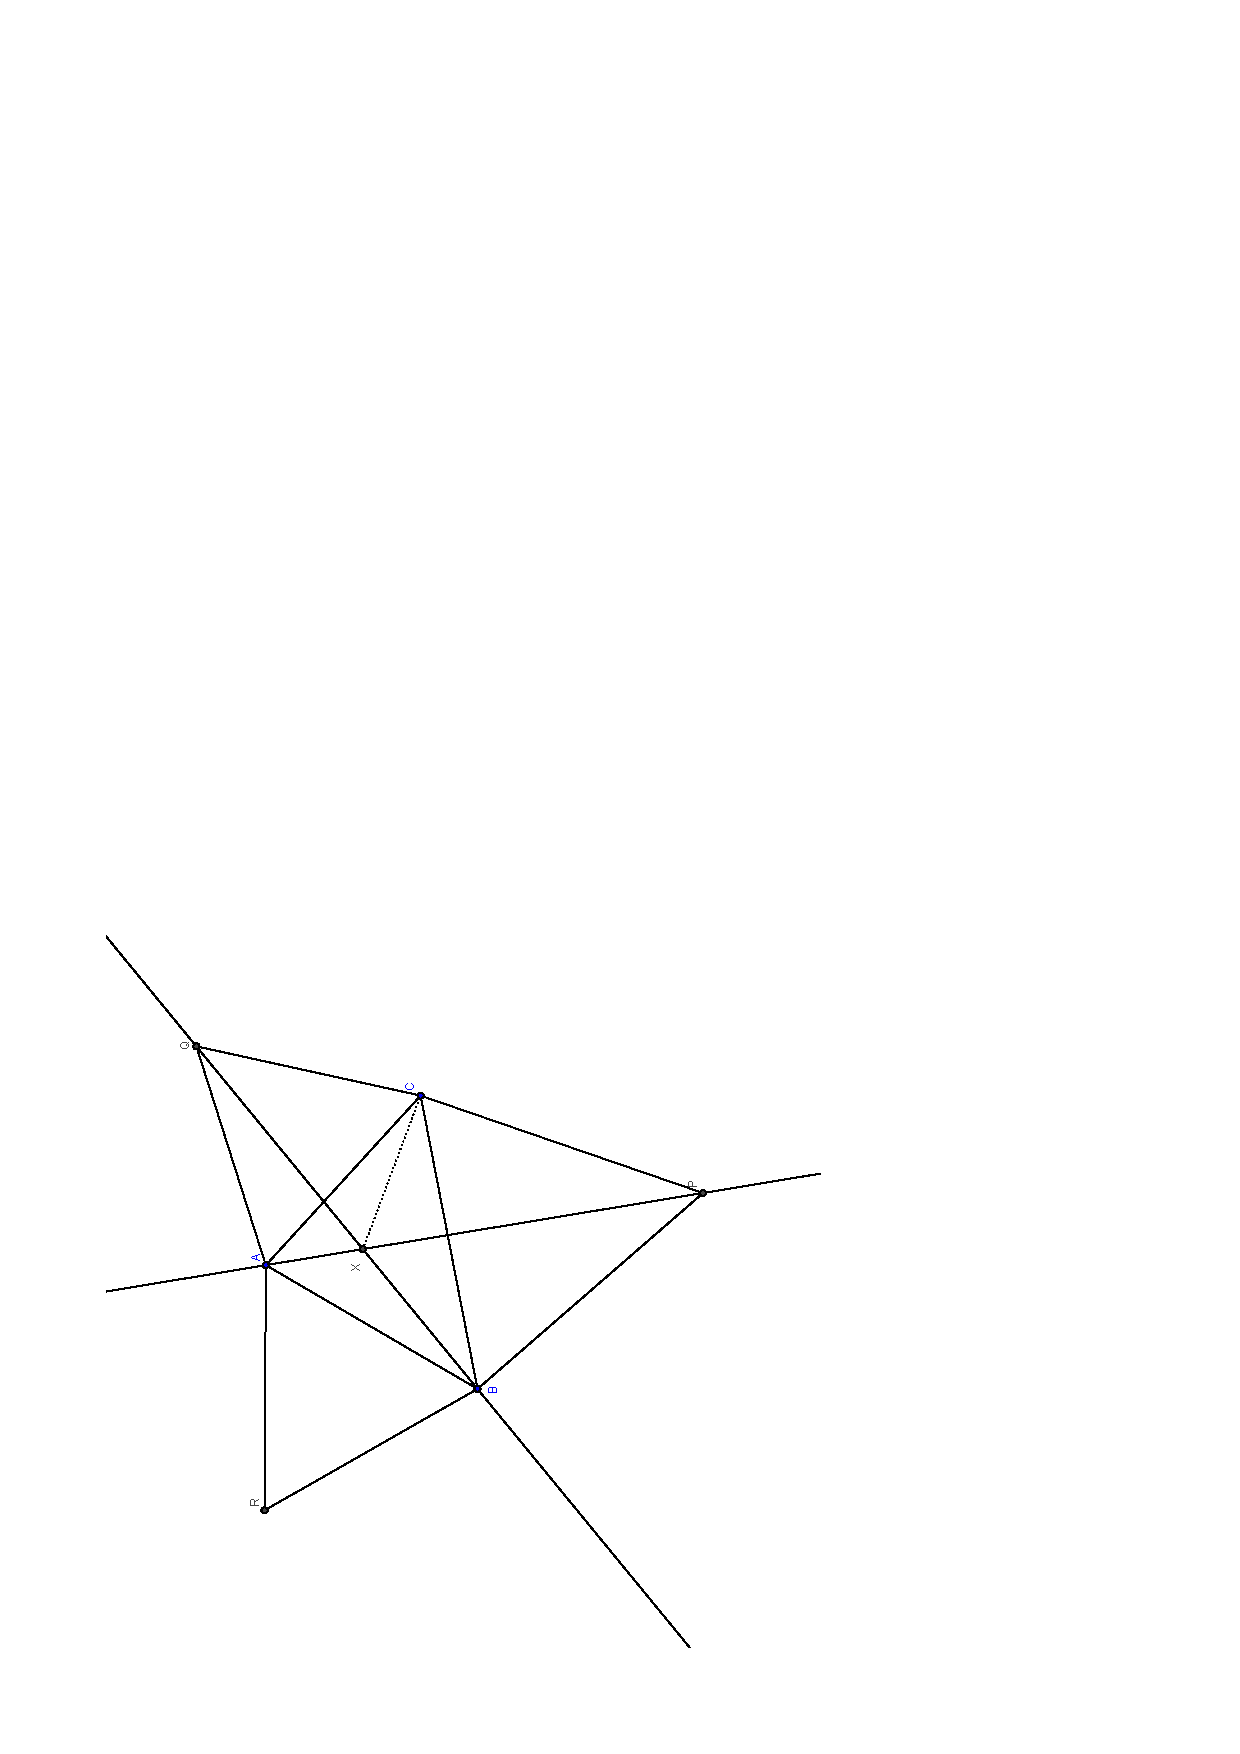
\includegraphics[viewport = 70 100 350 370, width = .45\textwidth, angle = 270, clip]{20151224-fig5.pdf}
\begin{picture}(0, 0)
\put(-32.5, -28){\circle*{3}}
\put(-106, -53){\circle*{3}}
\put(-145, -120){\circle{3}}
\put(-81.5, -198){\circle{3}}
\end{picture}} \hfil
\scalebox{0.9}{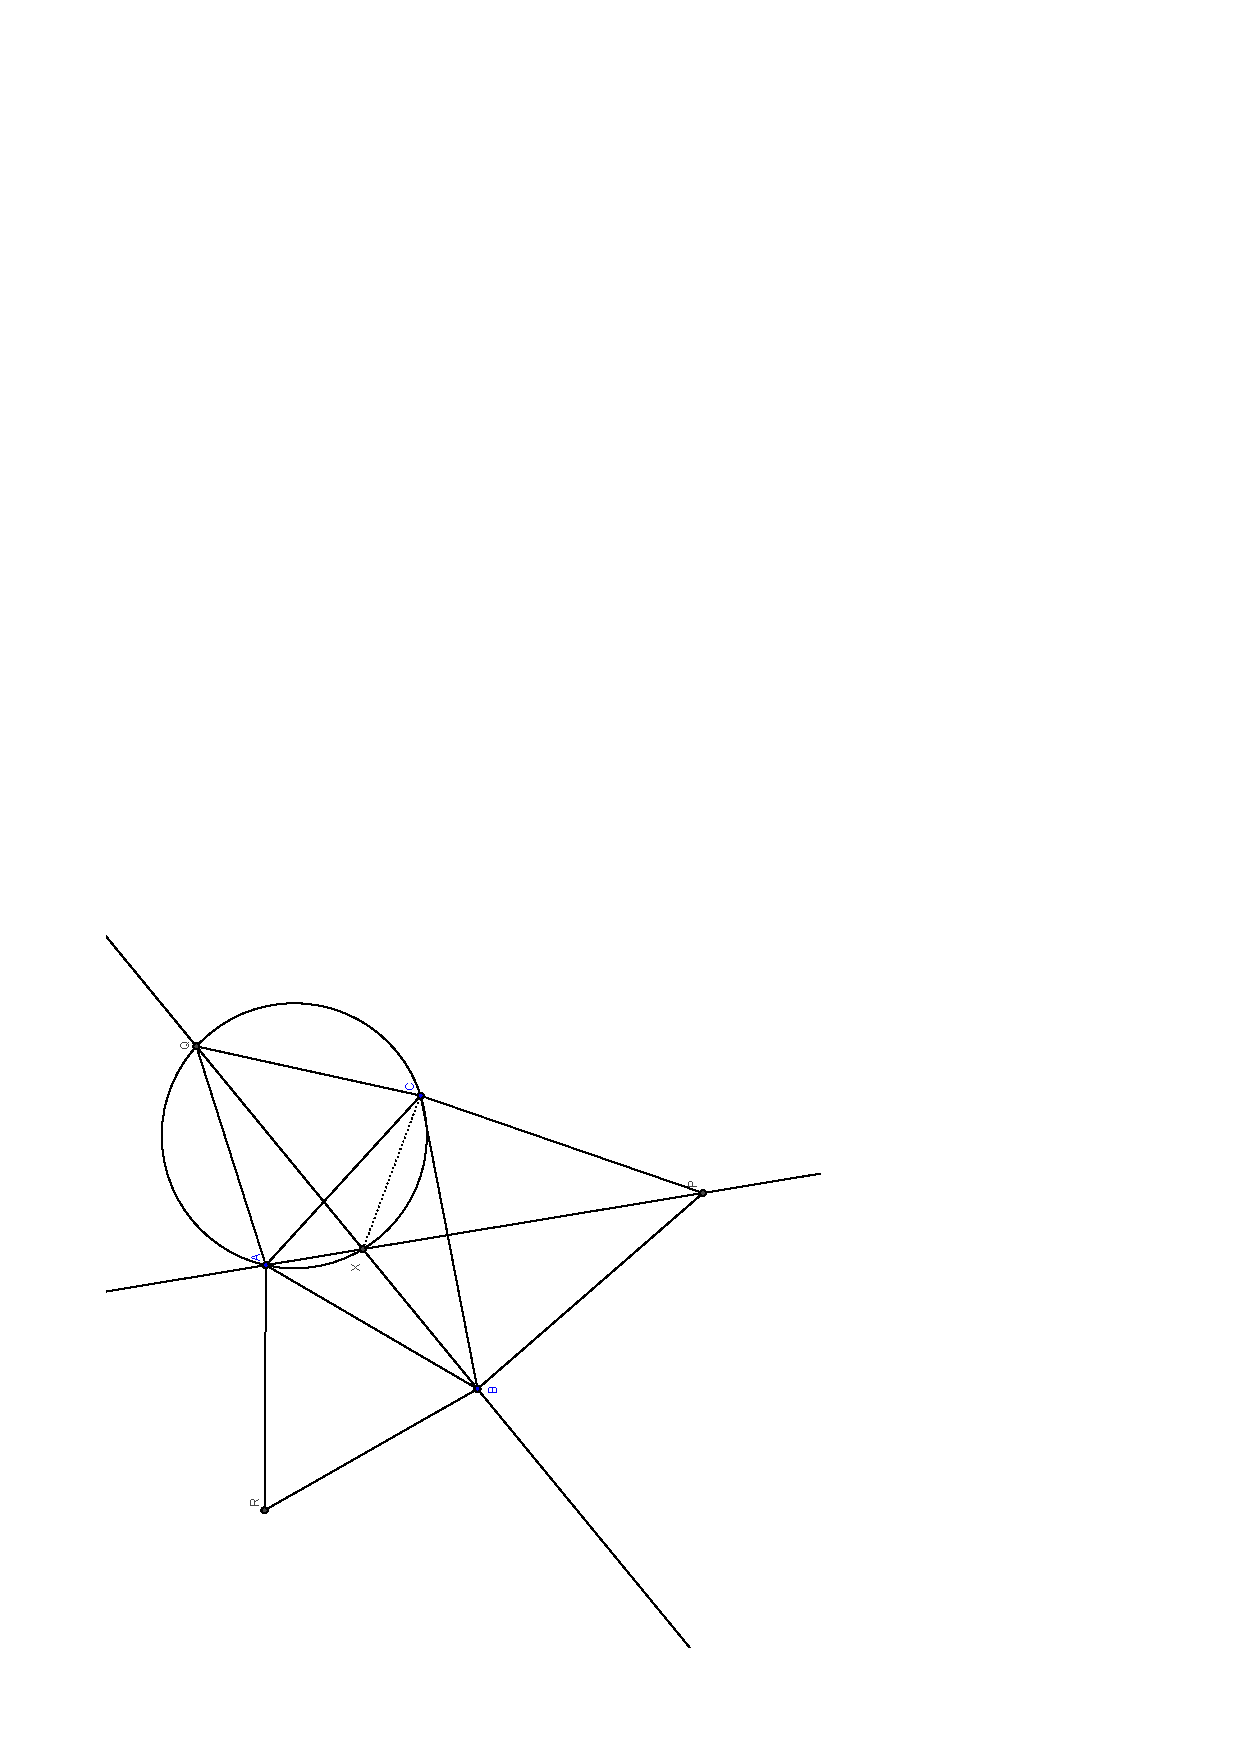
\includegraphics[viewport = 70 100 350 370, width = .45\textwidth, angle = 270, clip]{20151224-fig6.pdf}
\begin{picture}(0, 0)
\put(-32.5, -28){\circle*{3}}
\put(-106, -53){\circle*{3}}
\put(-145, -120){\circle{3}}
\put(-81.5, -198){\circle{3}}
\put(-39, -26){\framebox(2,2){}}
\put(-60.5, -96){\framebox(2,2){}}
\end{picture}}
\end{figure}

今度は直線$\mathrm{BQ}$と直線$\mathrm{CR}$の交点を$\mathrm{Y}$とします。先ほどと同様に$\bigtriangleup\mathrm{RAC} \equiv \bigtriangleup\mathrm{BAQ}$が示せます。これによって$4$点$\mathrm{A}$, $\mathrm{C}$, $\mathrm{Q}$, $\mathrm{Y}$が同一円周上にあることが分かり、円周角の定理から$\angle\mathrm{AQY} = \angle\mathrm{ACY}$が従います。

\begin{figure}[h!tbp]
\centering
\scalebox{0.9}{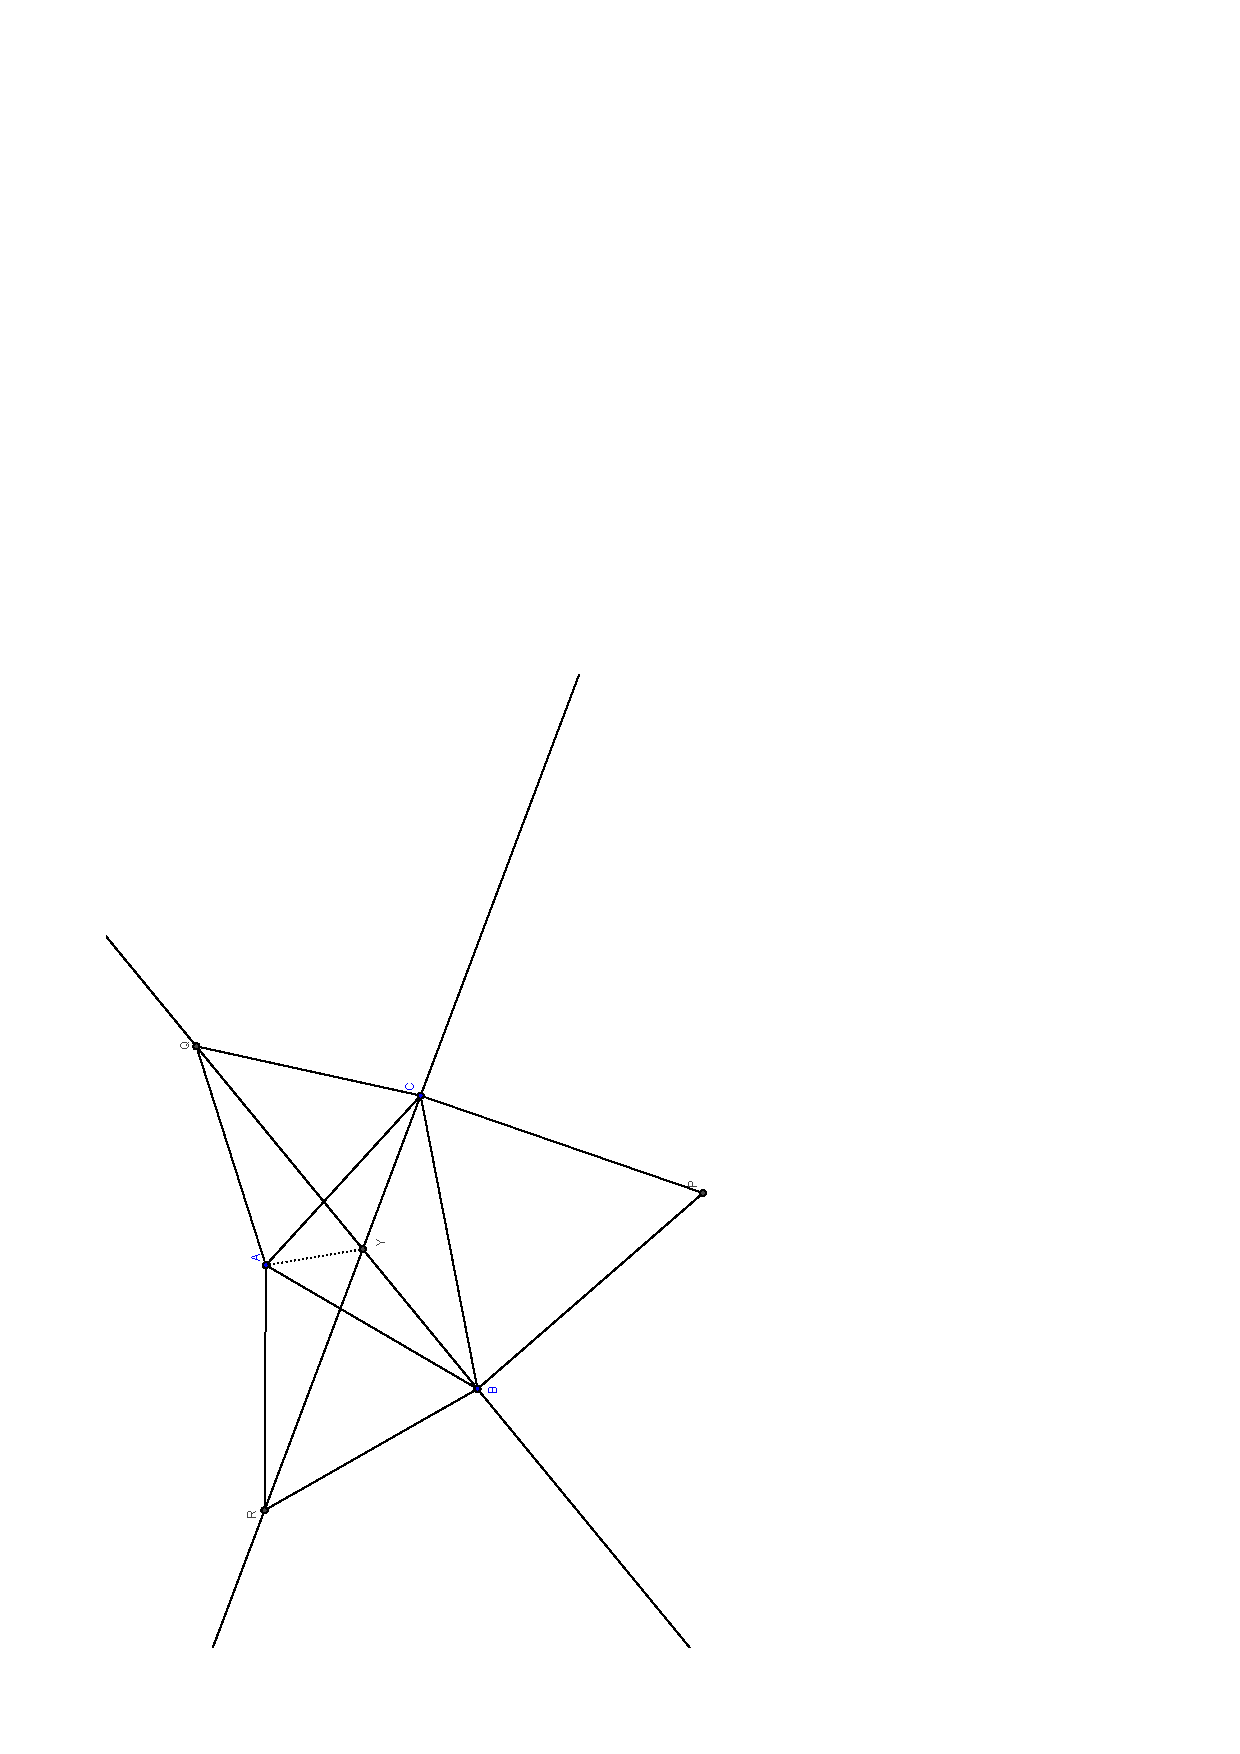
\includegraphics[viewport = 70 100 350 370, width = .45\textwidth, angle = 270, clip]{20151224-fig7.pdf}
\begin{picture}(0, 0)
\put(-39, -26){\framebox(2,2){}}
\put(-60.5, -96){\framebox(2,2){}}
\put(-185, -47){\line(1, -1){3}}
\put(-185, -50){\line(1, 1){3}}
\put(-144.5, -107){\line(1, -1){3}}
\put(-144.5, -110){\line(1, 1){3}}
\end{picture}} \hfil
\scalebox{0.9}{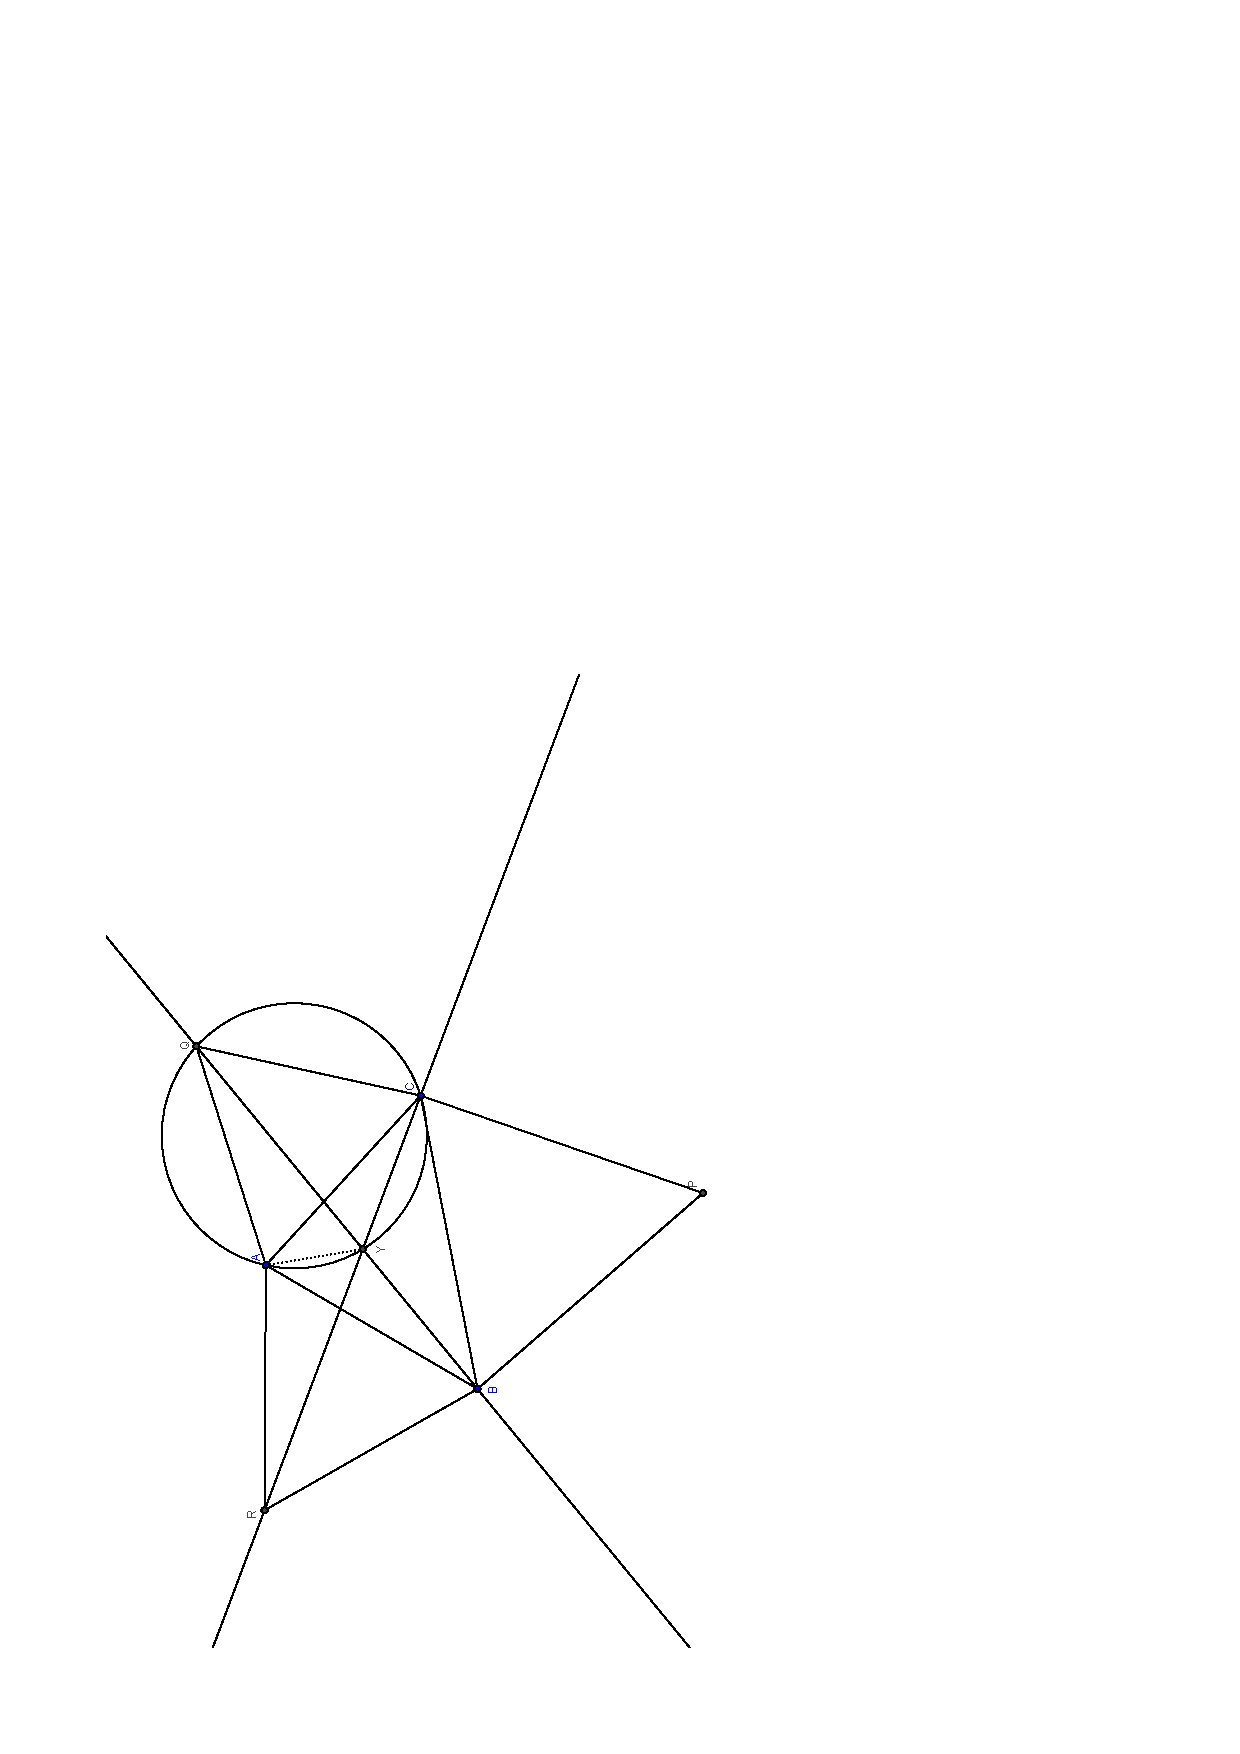
\includegraphics[viewport = 70 100 350 370, width = .45\textwidth, angle = 270, clip]{20151224-fig8.pdf}
\begin{picture}(0, 0)
\put(-39, -26){\framebox(2,2){}}
\put(-60.5, -96){\framebox(2,2){}}
\put(-185, -47){\line(1, -1){3}}
\put(-185, -50){\line(1, 1){3}}
\put(-144.5, -107){\line(1, -1){3}}
\put(-144.5, -110){\line(1, 1){3}}
\put(-32.5, -28){\circle*{3}}
\put(-106, -53){\circle*{3}}
\end{picture}}
\end{figure}

これらをまとめると、結局$\angle\mathrm{ACX} = \angle\mathrm{AQB} = \angle\mathrm{ACY}$と$\angle\mathrm{CAX} = \angle\mathrm{CQB} = \angle\mathrm{CAY}$が分かります。よって$2$角夾辺相等で$\bigtriangleup\mathrm{ACX} = \bigtriangleup\mathrm{ACY}$が従います。そして$\mathrm{X}$と$\mathrm{Y}$は共に$\bigtriangleup\mathrm{ABC}$の内部の点なので、$\mathrm{X} = \mathrm{Y}$でないといけません。これで示すべきことが言えました\footnote{ちなみにこの点は、Fermat点\index{Fermatてん@Fermat点}と呼ばれています。}。 \qed

\paragraph{図形的な解釈}

この問題の(1)と(2)は、なんとなく似ています。(1)は「$3$点が$1$直線上に乗る条件」で、(2)は「$3$直線が$1$点を通る条件」を考えています。そしてどちらについても、必要十分条件が行列式で書けています。これは決して偶然ではなく、必然的なものです。その理由を考えてみましょう。

キーポイントは\textbf{平面の問題を空間に持ち上げて考える}ことです。$3$次元空間内で$xy$平面に平行な平面$z = 1$を考えてみます。この平面に$\Pi$と名前を付けます。すると
\begin{itemize}
\item 空間$\mathbb{R}^3$内で原点を通り、方向ベクトルの$z$成分が$0$でない直線
\item 平面$\Pi$上の点
\end{itemize}
が$1:1$に対応します。実際$\Pi$上の点を取れば、原点とその点を通る直線がただ$1$つ存在します。逆に原点を通り方向ベクトルの$z$成分が$0$でない直線は、必ず平面$\Pi$と$1$点で交わります。同様にして
\begin{itemize}
\item 空間$\mathbb{R}^3$内で原点を通る、$xy$平面以外の平面
\item 平面$\Pi$上の直線
\end{itemize}
が$1:1$に対応します。実際、原点を通る$xy$平面以外の平面は必ず$\Pi$と交わり、その交わりが直線になります。逆に平面$\Pi$上に直線があれば、その直線と原点とを含む$\mathbb{R}^3$の平面がただ$1$つ存在します。かくして、元の問題を空間内で考えると、雑に言えば
\begin{itemize}
\item 平面$\Pi$上の点と、空間$\mathbb{R}^3$の原点を通る直線
\item 平面$\Pi$上の直線と、空間$\mathbb{R}^3$の原点を通る平面
\end{itemize}
とが対応することが分かりました\footnote{要は、原点を通る直線や平面を、原点から放射状に出た光源によって平面$\Pi$に射影している感じです。}。

こうすると嬉しいことがあります。$3$次元空間の場合、$\mathbb{R}^3$の原点を通る直線と原点を通る平面とが$1:1$に対応するのです。どう対応付けるのかは後回しにして、ここまでの事実を図式でまとめましょう。
\[
\begin{tikzcd}
\text{平面$\Pi$上の点} \arrow{d}{} & \text{平面$\Pi$上の直線} \arrow{d}{} \\
\text{$\mathbb{R}^3$の原点を通る直線} \arrow{u}{} \arrow{r}{} & \text{$\mathbb{R}^3$の原点を通る平面} \arrow{u}{} \arrow{l}{}
\end{tikzcd}
\]
この図式をぐるっと回ることで、平面$\Pi$上の点と平面$\Pi$上の直線が対応つきます。そうすると、この問題の(1)と(2)の条件が似ていることが自然な気が徐々にしてきます。

さて肝心の「$\mathbb{R}^3$の原点を通る直線と原点を通る平面との対応」ですが、これは難しくありません。
\begin{itemize}
\item 原点を通る直線には、それと垂直で原点を通る平面を
\item 原点を通る平面には、それと垂直で原点を通る直線を
\end{itemize}
対応させるだけです。この$2$つの対応が互いに逆向きなことは、明らかでしょう。$1 + 2 = 3$なので、$3$次元空間の場合では直線の次元と平面の次元を足したらちょうど空間全体の次元になります。このおかげで、直線と平面とが綺麗に対応づきます。

そして、この対応のすごいところは、単に「直線と平面が$1:1$に対応する」だけではありません。いま平面$\Pi$上で、異なる$2$直線が$1$点で交わっていたとします。このとき、今作った対応によって
\begin{itemize}
\item 交わる$2$直線のそれぞれを、対応する$\Pi$の点に
\item $2$直線の交点を、対応する$\Pi$上の直線に
\end{itemize}
それぞれ移すと、きちんと「$2$点が$1$直線上に乗っている図」が出てくるのです。その様子を絵にしてみました。
\begin{figure}[h!tbp]
\centering
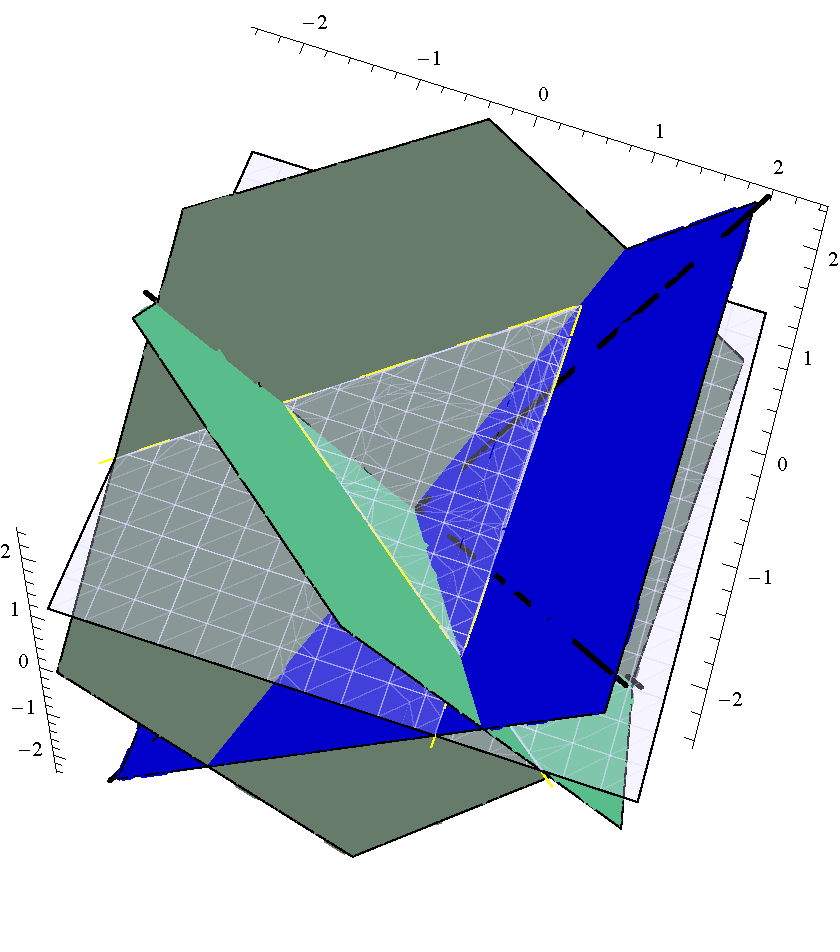
\includegraphics[width = .35\textwidth]{20151224-fig3.pdf}
 \hfil
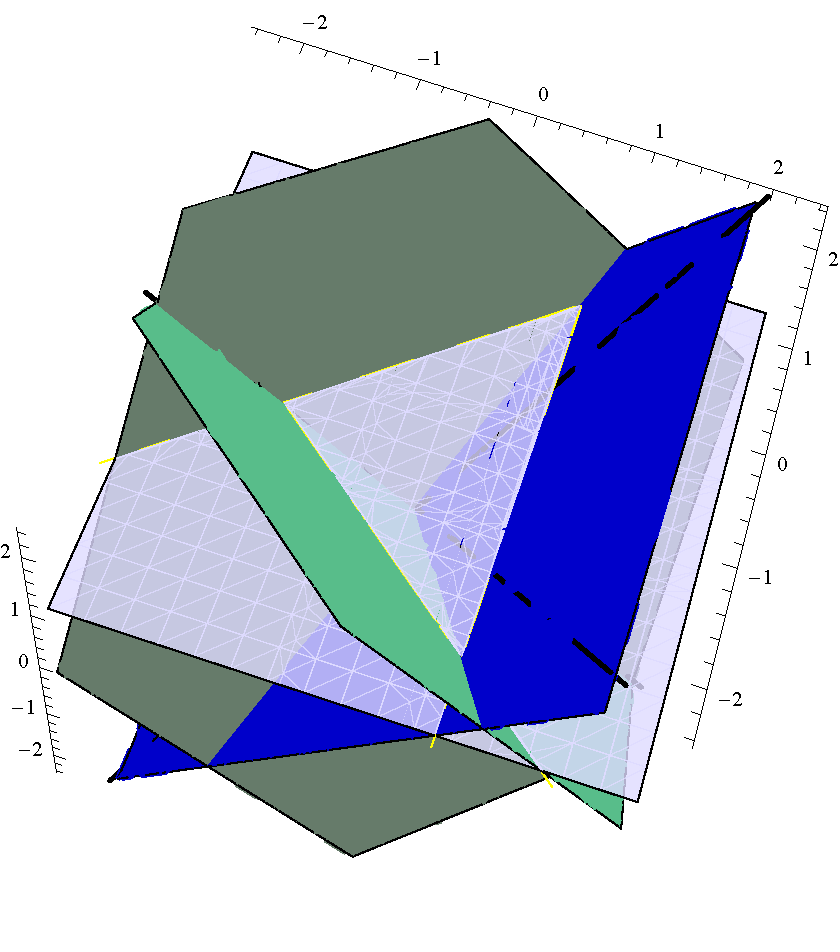
\includegraphics[width = .35\textwidth]{20151224-fig4.pdf}
\end{figure}

登場人物が多くてややこしい図なので、見方を説明します\footnote{\url{https://github.com/HideakiHosaka/2015_linear_algebra} に \texttt{duality\_between\_lines\_and\_planes.nb} という名前で、Mathematicaで	作った動くおもちゃを載せました。$2$枚の平面を色々な方向に動かしながら絵を見ると、何をやっているか分かりやすいはずです。大学のECCS端末にあるMathematicaで開いてみてください。}。まずは左の図からです。
\begin{itemize}
\item うっすらと半透明で描かれた平面が、$\Pi$です。
\item 左にある緑っぽい色\footnote{印刷はモノクロで行っていますが、元のPDFではカラーの図面になっています。「$3$枚の平面を左の$2$枚と右の$1$枚に分けて考える」ということさえ分かっていれば、原理的には分かるはず。ですが、できれば原本を見てください。}の$2$平面と平面$\Pi$との交わりにできる黄色い$2$直線が、今考えたいターゲットです。
\item 右側にある青い平面は、原点を通り、緑色の$2$平面の交線と垂直です。この青い平面の上に描かれた黒い$2$直線は、緑色の平面の法線です。
\end{itemize}
これを踏まえて、先ほどの対応を追いかけましょう。
\begin{itemize}
\item ターゲットの$2$直線の交点は、緑色の$2$平面の交線、それと垂直な青い平面を経由して、青い平面と半透明の平面$z = 1$の交わりにできる黄色い直線に対応する
\item ターゲットの$2$直線は、それぞれ緑色の平面およびその法線である黒い直線を経由して、黒い直線と平面$z = 1$の交点に対応する
\end{itemize}
というわけです。この対応を見れば、交わる$2$直線が$2$点を通る直線へとうつることが分かります。その理由も「緑色の$2$平面の交線と垂直な青い平面は、$2$平面それ自体とも垂直だから」だと分かります。また、右の図は平面$z = 1$の透け具合を減らして強調したものです。この白い平面の左側で交わる黄色い$2$直線が、青い平面上の$2$直線と白い平面の交点にそれぞれ移ります。

結局この対応を通せば、平面$\Pi$上で交わる$3$直線は、同一直線上にある$3$点に移ることが分かります。だから問題の(1)と(2)が似ているのは必然だと言えます。問題(1)と(2)のどちらかは真面目に解かないといけません。ですが(1)が解けていれば「(2)の条件は、今の対応で移し替えた後の$3$点が同一直線上に乗るための条件と同じ」という理由で、(1)に帰着できるのです。

\paragraph{双対原理と射影空間}

ちなみに、この問題のように「点と直線を入れ替えても正しい結果が得られる」という事実を\textbf{双対原理}\index{そうついげんり@双対原理}といいます。S2タームの最終回、p.~\pageref{section:dual_space}で双対空間の話を扱いました。双対空間を使うと、今の双対原理は「$\mathbb{R}^3$の原点を通る直線と、$(\mathbb{R}^3)^*$の原点を通る平面が$1:1$に対応する」と述べることができます。

さらに元々の問題では、原点を通る直線や平面を別の平面$\Pi$に射影していました。ですが射影をすると実はちょっとだけ不具合があります。$\Pi$上の点と直線は大体の場合は$1:1$に対応するものの、たまに「直線に対応する点が無限遠に飛んでいく」という不具合が生じるのです。この不具合を回避するには、射影をしないで物事を考える必要があります。このときに登場する「$\mathbb{R}^3$の原点を通る直線全体が作る空間」のことを、\textbf{射影空間}\index{しゃえいくうかん@射影空間}と呼びます。射影空間を用いることで、例外を一切なくした形で双対原理を述べることができるようになります。

こうした双対原理と射影空間の話は、西山亨『数学のかんどころ 19 射影幾何学の考え方』(共立出版) の6章を通じて丁寧に説明されています。初等幾何に限らず「双対」というアイデアは色々な場面で登場するものです。時間があったらぜひ読んでみてください。

\subsection{問題3: 行列の対角化}

行列を対角化する計算問題です。幸いなことに固有多項式の根が全てばらけるので、難しい処理は必要ありません。固有値と対応する固有ベクトルを求めるだけです。\\

\noindent (1) 行列
\[
A :=
\begin{pmatrix}
-3 & 2 & 1 \\
0 & 2 & 2 \\
0 & -1 & -1
\end{pmatrix}
\]
の固有多項式は
\[
\varphi_A(t) = \det(tI - A) =
\det
\begin{pmatrix}
t + 3 & -2 & -1 \\
0 & t - 2 & -2 \\
0 & 1 & t + 1
\end{pmatrix}
=
(t + 3)
\det
\begin{pmatrix}
t - 2 & -2 \\
1 & t + 1
\end{pmatrix}
= t(t + 3)(t - 1)
\]
と求まります。よって固有値は$-3, 0, 1$と分かります。$A$の形を見れば、固有値$-3$に属する固有ベクトルとして$\bm{v}_{-3} := {}^t(1, 0, 0)$が取れます。また固有値$0, 1$に属する固有ベクトルは、連立$1$次方程式$A\bm{x} = \lambda\bm{x}$ ($\lambda = 0, 1$)を解いて
\[
\bm{v}_0 =
\begin{pmatrix}
1 \\
3 \\
-3
\end{pmatrix}, 
\bm{v}_1 = 
\begin{pmatrix}
3 \\
8 \\
-4
\end{pmatrix}
\]
と求まります。かくして
\[
P:= 
\begin{pmatrix}
1 & 1 & 3 \\
0 & 3 & 8 \\
0 & -3 & -4
\end{pmatrix}
\]
とおけば、$P^{-1} A P = \diag(-3, 0, 1)$と求まります。

\noindent (2) 回転行列
\[
R(\theta) :=
\begin{pmatrix}
\cos \theta & -\sin \theta \\
\sin \theta & \cos \theta
\end{pmatrix}
\]
の固有多項式は$\varphi_{R(\theta)}(t) = t^2 - 2\cos \theta + 1$です。解の公式で解くと、根は
\[
t = \cos \theta \pm \sqrt{\cos^2\theta - 1} = \cos \theta \pm i \sin \theta
\]
だと分かります\footnote{本当は$\theta$の値に応じて$\sqrt{\cos^2\theta - 1}$が$\sin \theta$になるのか$-\sin\theta$のどっちになるのか変わります。ですが根号を外すときに$\pm$の符号がどっちになっても、「$2$つの根をまとめて$t = \cos \theta \pm i \sin \theta$と書ける」という事実に変わりはありません。なので少し横着した書き方をしました。}。これで固有値が求まりました。また連立$1$次方程式$R(\theta)\bm{x} = \lambda \bm{x}$ ($\lambda = \cos \theta \pm i \sin \theta$) を解いて、対応する固有ベクトルは
\[
\begin{pmatrix}
\cos \theta & -\sin \theta \\
\sin \theta & \cos \theta
\end{pmatrix}
\begin{pmatrix}
i \\
1
\end{pmatrix}
=
(\cos\theta + i \sin \theta)
\begin{pmatrix}
i \\
1
\end{pmatrix}, \quad
\begin{pmatrix}
\cos \theta & -\sin \theta \\
\sin \theta & \cos \theta
\end{pmatrix}
\begin{pmatrix}
-i \\
1
\end{pmatrix}
=
(\cos\theta - i \sin \theta)
\begin{pmatrix}
-i \\
1
\end{pmatrix}
\]
と求まります\footnote{固有多項式が重根、つまり$\theta = 0, \pi$の場合もこの式は正しいです。}。そこで
\[
P :=
\begin{pmatrix}
i & -i \\
1 & 1
\end{pmatrix}
\]
とおけば、$P^{-1} R(\theta) P = \diag(\cos\theta + i\sin \theta, \cos\theta - i \sin\theta)$が得られます。 \qed

\subsection{問題4: 実対称行列の対角化}
実対称行列
\[
A =
\begin{pmatrix}
0 & 0 & 1 \\
0 & -1 & 0 \\
1 & 0 & 0 
\end{pmatrix}
\]
を対角化する問題です。実対称行列であることから、直交行列によって対角化できることが分かります。

まず固有多項式は、$\det$を$2$行目について余因子展開すると
\[
\varphi_A(t) = \det(tI - A) = 
\det
\begin{pmatrix}
t & 0 & -1 \\
0 & t + 1 & 0 \\
-1 & 0 & t 
\end{pmatrix}
=
(t + 1)
\det
\begin{pmatrix}
t & -1 \\
-1 & t 
\end{pmatrix}
= (t + 1)(t^2 - 1)
= (t - 1)(t + 1)^2
\]
となります。よって$A$の固有値は$1, -1, -1$です。

次に固有ベクトルを求めましょう。$(\bm{e}_1, \bm{e}_2, \bm{e}_3)$を$\mathbb{R}^3$の標準基底とします。固有値$-1$に属する$A$の固有ベクトルとして、最初から$\bm{e}_2 = {}^t(0, 1, 0)$が見えています。すると残り$2$本の固有ベクトルは$\bm{e}_2$と直交するよう取れるはずなので、第$2$成分を持ちません。このことに注意すると、固有値$1$に属する固有ベクトルとして$\bm{v}_1 = {}^t(1, 0, 1)$が見つかります。最後に、外積で$\bm{e}_2, \bm{v}_1$の両方に直交するベクトルを作ると
\[
\bm{e}_2 \times \bm{v}_1 = \bm{e}_2 \times (\bm{e}_1 + \bm{e}_3) = \bm{e}_2 \times \bm{e}_1 + \bm{e}_2 \times \bm{e}_3
= -\bm{e}_3 + \bm{e}_1 = 
\begin{pmatrix}
1 \\
0 \\
-1
\end{pmatrix}
\]
となります。計算すると、予定通りこれが$A$の固有値$-1$に属するもう$1$本の固有ベクトルになっています。あとは、固有ベクトルの長さが$1$になるよう調整してから並べて
\[
P := 
\begin{pmatrix}
\frac{1}{\sqrt{2}} & 0 & \frac{1}{\sqrt{2}} \\
0 & 1 & 0 \\
\frac{1}{\sqrt{2}} & 0 & -\frac{1}{\sqrt{2}}
\end{pmatrix}
\]
とおけば、$P^{-1} A P = \diag(1, -1, -1)$となり、対角化が完了します。 \qed

\subsection{問題5: 平面上の$2$次曲線}

平面上で方程式$3x^2 - 2xy + 3y^2 = 4$が表す方程式を求める問題です。$xy$の項があるため、これは標準形の$2$次曲線を回転したものになっています。うまく回転させて、どういう形なのかをはっきりさせましょう。

\noindent (1) 実対称行列$A$を
\[
A =
\begin{pmatrix}
3 & -1 \\
-1 & 3
\end{pmatrix}
\]
で定めると、${}^t\bm{x} A \bm{x} = 3x^2 - 2xy + 3y^2$となります。よって方程式が${}^t\bm{x} A \bm{x} = 4$と書き換えられます。

\noindent (2) $A$の固有多項式は$\varphi_A(t) = t^2 - 6t + 8 = (t - 2)(t - 4)$なので、$A$の固有値は$2, 4$です。それぞれに対応する固有ベクトルは、連立$1$次方程式$A\bm{x} = \lambda\bm{x}$ ($\lambda = 2, 4$)を解いて
\[
\bm{v}_2 = 
\begin{pmatrix}
1 \\
1
\end{pmatrix}, 
\bm{v}_4 = 
\begin{pmatrix}
-1 \\
1
\end{pmatrix}
\]
と求まります。

\noindent (3) いま求めた固有ベクトル$\bm{v}_2, \bm{v}_4$は直交します。そこで長さを$1$に揃え、かつ$\bm{v}_2$から$\bm{v}_4$への向きが正の向きになるよう調整すると
\[
P := 
\frac{1}{\sqrt{2}}
\begin{pmatrix}
1 & -1 \\
1 & 1
\end{pmatrix}
\]
とおけば良いことが分かります。この$P$は$\pi/4$回転を表す回転行列で、$P^{-1} A P = \diag(2, 4)$を満たします。

\noindent (4) 元の方程式の左辺を、${}^tP = P^{-1}$を使って${}^t\bm{x} A \bm{x} = {}^t \bm{x} P P^{-1} A P P^{-1} \bm{x} = {}^t({}^tP \bm{x}) P^{-1} A P ({}^tP \bm{x})$と変形します。${}^tP \bm{x} = {}^t(u, v)$とおくと、$P^{-1} A P = \diag(2, 4)$より
\[
4 = {}^t\bm{x} A \bm{x} = 
\begin{pmatrix}
u & v
\end{pmatrix}
\begin{pmatrix}
2 & 0 \\
0 & 4
\end{pmatrix}
\begin{pmatrix}
u \\
v
\end{pmatrix}
= 2u^2 + 4v^2
\]
となります。よって$uv$座標系では、この曲線は$(u/\sqrt{2})^2 + v^2 = 1$と書けるので、$u$軸方向の長半径が$\sqrt{2}$, $v$軸方向の短半径が$1$の楕円だと分かります。

あとは$uv$座標系から$xy$座標系に変換すれば終わりです。$x, y$座標系を$u, v$座標系に変換するのに${}^tP = P^{-1}$を使ったので、$xy$座標系の基底を$uv$座標系の基底に変換する行列は$P$です。そして$P$が$\pi/4$回転を表す行列なので、$u$軸は${}^t(1, 1)$方向を、$v$軸は${}^t(-1, 1)$方向を向いていると分かります。これで曲線の概形が決まります。

\begin{figure}[h!tbp]
\centering
\begin{picture}(0,0)
\put(0, 86.1){\vector(1, 0){180}}
\put(88.8, 0){\vector(0, 1){175}}
\put(182, 83){$u$}
\put(92, 170){$v$}
\put(79, 78){$O$}
\put(147, 89){$\sqrt{2}$}
\put(-13, 90){$-\sqrt{2}$}
\put(90, 144){$1$}
\put(90, 22){$-1$}
\end{picture}
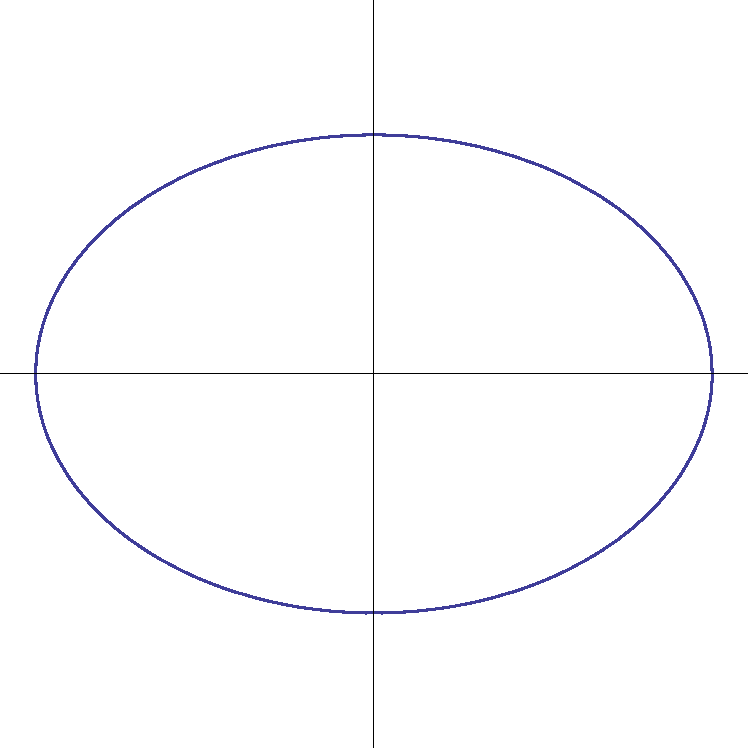
\includegraphics[width = .35\textwidth]{20151224-fig1.pdf}
 \hfil
\begin{picture}(0,0)
\put(0, 86.1){\vector(1, 0){180}}
\put(88.8, 0){\vector(0, 1){175}}
\put(88.8, 86.1){\vector(-1, 1){80}}
\put(88.8, 86.1){\line(1, -1){80}}
\put(88.8, 86.1){\vector(1, 1){80}}
\put(88.8, 86.1){\line(-1, -1){80}}
\put(88.8, 86.1){\dashbox(54.7, 54.7){}}
\put(73, 78){$O$}
\put(182, 83){$x$}
\put(92, 170){$y$}
\put(170, 166){$u$}
\put(3, 167){$v$}
\put(137, 88){$1$}
\put(90, 133){$1$}
\end{picture}
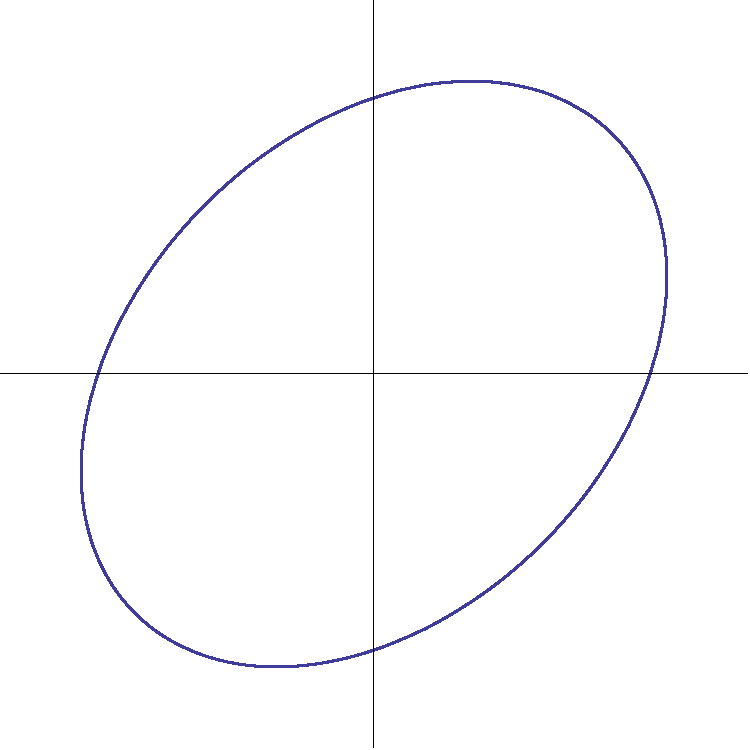
\includegraphics[width = .35\textwidth]{20151224-fig2.pdf}
\end{figure}

なお、回転の向きを逆向きにしていないかどうか心配になるかもしれないので、チェックしておきましょう。上の議論で$u$軸上の点$(\sqrt{2}, 0)$は曲線上に乗っています。もし回転のさせ方が正しければ、この点は$xy$座標系で$(1, 1)$という点に対応するはずです。そして元の方程式$3x^2 - 2xy + 3y^2 = 4$に$x = y = 1$を代入すると式が成り立ちます。これで、回転のさせ方が正しいと分かります。 \qed

\section{$1$年間の締めくくり}

それでは最後に、$1$年間の授業の締めくくりをします。これまでの授業内容をおさらいし、そして線型代数の後に続く数学を覗いてみましょう。

\subsection{これまでにやったこと}

この$1$年間で何をやったのか、簡単におさらいします。ここに書いてあることがすらすら納得できれば、線型代数の基礎は分かっていると思います。

\paragraph{行列の演算}

数を縦に$m$個、横に$n$個並べたものを$(m, n)$型の行列といいます。この行列について
\begin{itemize}
\item $(m, n)$型の行列同士の足し算と引き算
\item $(m, n)$型行列と$(n, l)$型行列の掛け算
\end{itemize}
が定義されます。掛け算の規則は一見すると変わっていますが、後でこの掛け算は「行列を線型写像と思った時の合成」にぴったり対応すると分かります。また行列の掛け算には
\begin{itemize}
\item 順序がひっくり返せない
\item $O$でない行列同士の積が$O$になることがある
\item 「逆数」に当たる逆行列が必ずしも存在しない
\end{itemize}
という性質があります。こうした性質のおかげで、行列の掛け算は数の掛け算とかなり違う様子を示します。

\paragraph{線型空間と線型写像}

行列の理論を展開するにあたり、必要なのは「数ベクトル空間$\mathbb{R}^n$の上で、足し算とスカラー倍が定義されている」ということだけです。そこでこの性質だけを抜き出して抽象化して、\textbf{線型空間}が定義されます。標語的には「足し算とスカラー倍ができる集合」が線型空間です。そして「線型空間の構造と相性のいい写像」を考えることで、\textbf{線型写像}の概念が定義されます。数ベクトル空間の場合、線型写像と行列とは全く同じものを表します。

さて、線型空間の中には小さい線型空間が入っています。これらの空間を、親玉の線型空間の\textbf{部分空間}と呼びます。数ベクトル空間の部分空間がどんな形をしているか考察することで、線型空間が「原点を持つまっすぐな空間である」というイメージが浮かび上がります。そして部分空間を定義することで、線型写像にはもれなく$2$つの部分空間がついてくることが分かります。それは定義域の部分空間である\textbf{核}と、値域の部分空間である\textbf{像}です。核と像は、それぞれ線型空間の単射性と全射性を反映しています。単射性と全射性がそれぞれ核と像の大きさで測れるので、線型写像は極めて振る舞いの良い写像です。

そして線型空間を考える上で重要なのは、\textbf{基底}の存在です。数ベクトル空間に基底が存在するように、全ての線型空間は基底を持ちます。しかも一つの線型空間の中でどんな基底を持ってきても、同じ本数のベクトルからなります。その本数のことを線型空間の次元といいます。次元を用いると、たとえば「方程式の解の自由度」のような量を厳密に定式化できます。これでも十分利用価値がありますが、何より「線型写像の核と像の次元を足し合わせると、定義域の次元に一致する」という定理 (\textbf{次元定理}) が強力です。線型写像の単射性と全射性はそれぞれ核と像の次元で判定できるので、次元定理を組み合わせることで、自動的に線型写像の単射性/全射性が証明されることがしばしばあります。

\paragraph{行列を用いた連立$1$次方程式の解法}

連立$1$次方程式は行列の積を用いて$A\bm{x} = \bm{b}$の形に表すことができます。このとき、係数に現れる行列$A$を\textbf{係数行列}といいます。また係数行列$A$の右側に方程式の右辺のベクトル$\bm{b}$を並べてできる行列を、\textbf{拡大係数行列}といいます。係数行列を用いると、消去法による連立$1$次方程式の解法は「\textbf{基本行列}」と呼ばれる行列の積で表せます。基本行列が逆行列を持つことを合わせると、消去法を用いて正方行列の逆行列を計算するアルゴリズムが得られます。

また連立$1$次方程式を行列で$A\bm{x} = \bm{b}$と表しておくと、線型空間と線型写像の言葉が使えるようになります。$A\bm{x} = \bm{b}$が解を持つことは、$\bm{b}$が線型写像$A$の像に入ることと同値です。このことを次元で言い換えることもできます。行列を線型写像と思った時、像の次元を行列の\textbf{階数}といいます。すると連立$1$次方程式が解を持つことは、係数行列と拡大係数行列の階数が一致することと同値です。

\paragraph{行列式の計算}

行列式とは$n$次正方行列に対して定義される数です。$n$次正方行列を$n$本の数ベクトルと思ったとき、「$n$本のベクトルが張る平行$2n$面体の向き付けられた体積」が行列式です。$n$本のベクトルが$1$次従属なことと、それらが張る平行$2n$面体の体積が$0$なことは同値です。したがって行列式が$0$かどうかで、$n$本のベクトルの$1$次独立性、あるいは同じことですが行列の正則性を判定できます。

この行列式は色々な公式を持ちます。たとえば行列式は、$n$個の文字にわたる置換の和として明示的に書き下す公式を持ちます。\textbf{交代性}と\textbf{多重線型性}という性質によっても、行列式を特徴づけることができます。また、$n$次の行列式を$(n - 1)$次の行列式の計算に落とし込む\textbf{余因子展開}の公式を使っても行列式は計算できます。これらの公式を的確に使うことが、行列式を手際よく計算する鍵です。

\paragraph{内積と正規直交基底}

ここまでの議論ではベクトルの足し算とスカラー倍しか使ってきませんでしたが、数ベクトル空間にはもう一つ「\textbf{内積}」という演算が備わっています。$3$次元空間における内積は、$n$次元の数ベクトル空間に対しても一般化できます。したがって$n$次元のときでも数ベクトル$2$本が直交することと、数ベクトルの長さが定義できます。このとき「全て長さが$1$で、どの$2$本の組合せも直交する」という良い条件を満たす基底を\textbf{正規直交基底}といいます。また正規直交基底のベクトルを並べてできる行列は、\textbf{直交行列}と呼ばれます。

\paragraph{固有値と対角化問題}

$n$次正方行列を$\mathbb{R}^n$のベクトルに当てると、	同じ空間の中で別のベクトルへと変化します。このとき普通はベクトルの向きが変わりますが、運が良いと向きは変わらず、長さだけが変化することがあります。こういうベクトルを\textbf{固有ベクトル}といいます。そして固有ベクトルからなる基底を作ることができると、新しい基底に関して元の行列が対角行列で表示されます。この操作を行列の対角化といいます。対角化を求めるには、まず\textbf{固有多項式}を計算し、その根である\textbf{固有値}を求めます。その後、それぞれの固有値に属する固有ベクトルを求めます。

行列の固有値が全部バラバラであれば、行列は対角化可能です。しかし固有値に重複が出てくると、対角化ができない場合があります。この問題の本質的な理由は「固有値が全て$0$である巾零行列は、必ずしも行列のサイズと同じ本数の固有ベクトルを持つとは限らない」という事実です。そのような場合は次善の策として、対角線の上にいくつか$1$が並んだ\textbf{Jordan標準形}という形にまで変形ができます。

\paragraph{Hermite行列のユニタリ対角化}

一般に行列は対角化可能とは限らないわけですが、実対称行列やHermite行列の場合、必ず対角化可能になるという事実があります。この理由は一言で言えば「標準内積との相性が良い」ということに尽きます。しかも対角化のときに挟む行列として、実対称行列が相手なら直交行列が、Hermite行列が相手ならユニタリ行列が取れるのでした。対角化するだけなら別に直交行列やユニタリ行列を使わなくてもいいですが、実対称行列やHermite行列の対角化可能性を示す際には\textbf{Gram--Schmidtの正規直交化法}が必要で、その証明を見ると「直交行列やユニタリ行列が持ってこられる」ということが分かります。

\paragraph{平面内の$2$次曲線}

$2$つの変数$x$と$y$の実$2$次式 ($2$次形式) は、実対称行列を用いて表すことができます。そして、実対称行列はいつでも直交行列で対角化できるのでした。そこで$2$次形式に現れる実対称行列を対角化すると、ややこしい$2$次形式を$2$次曲線の標準形に変形できます。これによって、座標軸に対して斜めった楕円、双曲線や放物線がどういう格好をしているのかを突き止めることができます。

\subsection{やり残したこと}

$1$年間の授業を通してずいぶん色々なテーマが扱われましたが、実はまだ少しだけ、取りこぼしがあります。それを$2$つほど補足しておきます。

\paragraph{小行列式}

(正方とは限らない) 行列の中からちっちゃい正方行列を切り取ってくると、その行列式を計算できます。これを元の行列の\textbf{小行列式}といいます。今年の授業では行列式の登場が遅めだったので、小行列式の出番がありませんでした。でも実は、中々使える道具です。

小行列式が役立つ$1$つの場面は、$1$次独立性の判定です。何本かベクトルが与えられたとき、その一部の成分を抜き出したものが$1$次独立になっていたら、元のベクトルたちも$1$次独立です。また、$n$本の$n$次元数ベクトルの$1$次独立性は行列式が$0$でないことと同値です。だからたとえば、数ベクトルを何本か並べた時に、明らかに行列式が$0$じゃない小行列 (たとえば三角行列とかVandermonde型の行列) が見えれば、直ちに$1$次独立だと判定できます。

S2タームの終わりの方で取り組んだ「線型写像の核や像の基底を求める」という問題で、この方法は特に有効です。基底を求めるには、$1$次独立なベクトルを探さないといけません。当時は頑張って連立$1$次方程式を解いていたわけですが、行列式を知っていればもっと計算を短絡させられます。復習するときに、ぜひ小行列式のことを頭に置いて計算してみてください。

\paragraph{直和}

基底を使うと、線型空間を「基底の方向」に分けることができます。が、時と場合によっては基底を使るまでしなくても、線型空間を「いくつかの部分空間の方向」に分けられれば十分なことがあります。こういうときに役立つのが、線型空間の直和です。この解説プリントではあまり直和を真面目に扱わなかったので、直和が必要な場面でも、基底を取ることで直和の利用を回避していました。ですが、直和の性質をきちんと調べた上で使いこなす方が、議論の筋は良いです。各自で本を読んで勉強してください。

\subsection{参考書案内}

ここまでまとめた内容を復習するのに、また一歩踏み込んだ内容を勉強するために、TAの穂坂の主観でいくつか線型代数の本を紹介します。手元にあって読んだことがある本のみを紹介しているので、紹介の仕方には偏りがあると思います。他にも世の中には良い本があるはずなので、一つの意見として受け止めてください。

\begin{itemize}
\item 佐武 一郎『線型代数学』(裳華房)
\item 足助 太郎『線型代数学』(東京大学出版会)
\item 長谷川 浩司『線型代数』(日本評論社)
\item 斎藤 毅『線形代数の世界』(東京大学出版会)
\item 室田 一雄・杉原 正顯『線形代数I』(丸善)
\end{itemize}

一押しは佐武一郎先生の『線型代数学』(裳華房) です。初版の出版年は1974年と中々古い本ですが、最近新装版が出ました。僕は学部$1$年生のとき、この本で線型代数を勉強しました。線型代数の基本的なことが一通り書かれているのはもちろんですが、各章の終わりに「研究課題」という節がついており、発展的なテーマが扱われているのが嬉しいところです。何度読み返しても味わいがあります。

もう少し新しく書かれた教科書として、足助先生と長谷川先生の本を紹介します。お二人とも現役の数学者で、足助先生の方は駒場キャンパスにある数理科学研究科に、長谷川先生は東北大学にいらっしゃいます。どちらの本も、この$1$年の授業で扱ったような基礎的なことは全て書かれており、程よく応用的な話も書かれています。$2$冊を比べると、長谷川先生の本は平たい書き方である一方、足助先生の本は「いかにも数学書らしい本」という感じがします。人によって好みは別れるでしょう。

斎藤毅先生も、駒場キャンパスにある数理科学研究科の先生です。斎藤先生の『線形代数の世界』は他の本と違い「大学$1$年生で線型代数を習った人が、より高度な線型代数の理論を学ぶための本」です。「高度な線型代数」をうたった本の大半は、線型代数よりさらに話を広げた「環上の加群の理論」というものを扱うのですが、この本は珍しく線型代数の範囲で収まっています。

最後に挙げた室田先生と杉原先生の『線形代数I』は、東京大学工学教程というシリーズのうちの$1$冊です。工学部の先生方が執筆されただけあって、書き方はかなり工学寄りです。諸々の定理が成り立つ原理に関する記述が深くない一方、工学の中で線型代数がどう使われるかについては、豊富に例が扱われています。工学での例を知るには非常に良い$1$冊でしょう。他の本と組み合わせて勉強することをお勧めします。

\subsection{この後に続く数学}

最後に、$1$年生の授業に続く数学をちょっとだけ紹介します。「もう数学勉強するの嫌だ」という気持ちの人もいるかもしれませんが、少しだけ聞いてください。

実は数学を専門としない限り、\textbf{この先の人生で必要になる数学は大体$1$年生の勉強で事足ります}。希望する専門分野があるなら、その分野の大学院の入試問題を見てみると良いでしょう。多分、一般教養科目として「数学」がありますが、そこに並んでいる問題の多くは微積分か線型代数です。実際に必要になる計算テクニックの多くは、既に皆さんが勉強した内容でカバーできるのです。

もちろん理論物理や電気工学など、ジャンルによっては高度な数学が必要になることもあるでしょう。そこで以下、大事と思われる順に、この先に出てくる数学を紹介します。

\paragraph{微分方程式}

これはほとんど全ての人にとって必修です。自然科学ならまず間違いなく、「時間が経つにつれて連続的に変化する量」を分析する必要性に迫られます。たとえば地球と太陽の距離とか、化学反応の進行する速度とか、生体内で代謝されるホルモンの量とか。そして、こうした連続量が従う法則は、ほぼ確実に微分方程式で記述されます。こういう事情で、微分方程式が必要になるのです。

微分方程式にも色々難しい理論がありますが、高度なことを知る必要はないでしょう。現実問題として、積分で解ける微分方程式はごくわずかしかなく、解けない大多数の方程式は計算機によって近似的に処理されます。ですから変数分離形など、いくつか有名な方程式を解けるようになっていけば当面事足ります。$2$年生になったら微分方程式の授業があるはずですので、頻出問題の解き方だけはぜひ学んでください。

\paragraph{ベクトル解析}

ベクトル解析は、平面や空間内のベクトル値函数を対象にした微積分の理論です。ベクトル値函数は単なる函数という以上に、空間の各点にベクトルが張り付いた「場」という意味を持ちます。たとえば物理学では、万有引力の場や電場・磁場といったものが典型的な例です。このような「場」を表す函数に対しては、偏導函数を上手く使うことで「湧き出し」や「回転 (渦)」を調べることができます。また場が与えられると、線積分・面積分といった特別な積分が考えられます。こうした「場」に固有の事情を調べるのが、ベクトル解析の主目的です。

\paragraph{複素函数論}

$1$年生で習う微積分では実変数の函数を扱いましたが、複素函数論では、$1$変数の複素数変数の函数を扱います。複素変数$1$個は実変数$2$個と等価なので、ちょっと考えると「$2$変数のベクトル値函数と何が違うんだろう」と思うかもしれません。ですが「複素函数の微分」を上手く定義すると「微分可能」という条件が程よく強くなり、微分可能な函数が非常に良い性質を示すようになるのです。こういう函数を\textbf{正則函数}といいます。

そして複素函数に対しても、積分をすることができます。特に正則函数や、あるいはいくつか発散する点を許した有理型函数と呼ばれる函数は\textbf{留数定理}と呼ばれる定理を満たします。実はこの留数定理が、普通の実$1$変数函数の積分を計算するのに役立つことがあります。おそらく今ある汎用的な積分公式の中で、最後に学ぶのが留数定理でしょう。

\paragraph{群論}

図形や式の持つ「対称性」を抽出して得られる概念が、群と呼ばれるものです。線型代数の授業の中では、$n$次対称群$\mathfrak{S}_n$や、正則行列のなす群$GL_n(\mathbb{R})$などが登場しました。こういう群の性質をもっと深く探るのが群論です。

大学入試の問題とかでも、数学の問題を解くときに「対称性」を使ったことは何回かあるのではないかと思います。群論を使うという行為は、ある意味で「対称性」を使った問題の解き方を一段と推し進めることにあたります。ですから非常に強力です。たとえば量子力学では、水素原子の波動関数を求めるのに回転対称性をフル活用します。水素原子に限らずもっと大きな分子でも、対称性の解析で軌道エネルギーの縮退度を決定できたりします。またX線回折による結晶解析では、どういう対称性がどういうX線反射パターンを生み出すかという情報を用います。この「結晶の持つ対称性」の分析は、空間群と呼ばれる群を調べることに他なりません。

\paragraph{Fourier級数}

電気回路や音響など「波」を扱う上で必須の理論です。このプリント中でも一度だけ、直線$y = x$を閉区間$[-\pi, \pi]$の上で三角函数の和で表す式をp.~\pageref{paragraph:Fourier_series}で紹介しました。この話をもっと深く追求し、あらゆる周期関数を簡単な三角函数の無限級数で表すのが、Fourier級数です。

Fourier級数は、周期的な函数を「色々な周波数の単純な波」に分解してくれます。たとえば音なら空気の振動を、電気信号なら電流/電圧の波を、Fourier級数展開によって単純な波にバラせます。これにより音の響き方や電気回路の応答といった現象を調べるのに「単純な波に対する振る舞いを調べておいて、後でそれらを重ね合わせる」といった手法が使えます。

\subsection{最後に: 編集後記}

ちょっとだけ紙面が余ったので、$1$年間線型代数のTAをしてみての感想とかを書きます。

\paragraph{「理論 vs 計算」の問題}

この解説プリントを作るとき、いつも念頭に置いていたのは「どの程度理論的に掘り下げるか」という問題です。理学部数学科の人が相手なら、みんな抽象的な数学が好きですから、がっつり理論的な数学をすれば大丈夫です。しかし皆さんの中では、理論数学が好きな人は少数派でしょう。実際提出されたレポートを見ていると、計算問題が出た回だけ明らかに提出量が増えていました。

確かに「計算で済むならそれでよい」という考え方は一理あります。難しい理論を勉強するのは大変ですし、計算だけが目的なら、わざわざ面倒なことをする必要もないでしょう。ただ理論が計算に役立つことも事実です。理論を知っていることは、計算を手際よく行う上でも、また計算ミスをなくす上でも役立ちます。理論ばかり勉強しても計算は進まない、一方で理論を知ってる方が計算しやすい。コンピュータの利用を踏まえても、この事実は変わりません。目的に応じて「どこまで理論に首を突っ込むのが最適か」を考える必要があるのです。

どこに最適点があるかはケースバイケースです。ですが個人的には、$1$年生の線型代数で学ぶことくらいは、原理まで込めて分かっていた方がいいような気がしています。だから解説プリントでは、なるべく「理論をどう計算に使うか」を説明しようと頑張ったつもりです。皆さんにそうしたテクニックが上手く伝えられてたら、よいのですが……。

\paragraph{線型代数の奥深さ}

今回プリントを作るにあたって、実は「何も本を見ないで、一から証明を書き下そう」というチャレンジをしていました。中々大変でしたが、このチャレンジを通じて、色々な面で「線型代数は奥深い」という事実を感じることができました。定理一つとっても、証明のやり方は複数通りあるのが普通です。話を一から組み立てるには「今の前提知識は何か、それを踏まえてどういう証明をするのが筋が良いか」を考えないといけません。また、複数の証明法を考えると「各々の証明の限界はどこにあるのか」が見えてきます。中々良い頭の訓練になりました。

それから線型代数より少し先の数学を知っていると、線型代数が広がりを持っていることが良く見えます。演習問題中に面白いネタが登場したときは、なるべく背景に対する解説を入れるようにしました。また、その中でも特に難しめのネタは「おまけ」として扱いました。何か$1$つでも、面白いと思ってもらえるものがあったら嬉しいです。ただ「おまけ」で扱った内容は、正直難しすぎたかなという気もします。すいません。\verb|(^^;)|

\paragraph{数学の景色}

よく「数学をすることは、ある意味で山登りに似ている」と言われます。数学では命題を一つ一つ積み重ねて、大きい定理へと近づいていきます。こうしたところは、山を一歩一歩登ることと似ています。また「振り返ったときの景色の良さ」も数学と山登りとで似ているところです。ある程度数学の理解が進んでから昔の復習をすると、一つ一つの命題・定義の意味が良く見渡せるようになります。

そして「昔やったことを振り返ると良く分かる」というのは、きっと、数学に限った話ではありません。これから先皆さんは (おそらく、数学とは異なる) 専門の学科に進んで色々なことを知ると思います。その際、たまに過去のことを振り返ってみてください。昔に勉強したことが一段と良く分かるようになっているはずです。そうして理解を深めることが、次の一歩を踏み出す原動力の一つになるでしょう。

この先学術的なことでもそれ以外のことでも、色々大変だとは思いますが、こつこつと頑張ってください。皆さんの大学生活での積み重ねが、実りあるものになりますように。

